\documentclass[11pt,a4paper]{article}

% ---- Packages ----
\usepackage[margin=1in]{geometry}
\usepackage{amsmath,amssymb,amsfonts}
\usepackage{graphicx}
\usepackage{booktabs}
\usepackage{hyperref}
\usepackage{cite}
\usepackage{caption}
\usepackage{subcaption}
\usepackage{enumitem}
\usepackage{float}
\usepackage{xcolor}
\usepackage{multirow}
\usepackage{array}
\definecolor{darkgreen}{rgb}{0.0,0.5,0.0}
\definecolor{darkred}{rgb}{0.6,0.0,0.0}

% ---- Metadata ----
\title{\vspace{-1.5cm}Modern Neural Methods for the Traveling Salesman Problem\\
\large Reproduction, Benchmarking, and Original Improvements}
\author{Pan Qiao\\
\texttt{CS240: Delivery Route Optimization in Modern Logistics}}
\date{June 2026}

\begin{document}
\maketitle

\begin{abstract}
This report presents a comprehensive study of modern neural approaches to the Traveling Salesman Problem (TSP), organized around the reproduction of two recent methods---DIFUSCO (NeurIPS 2023) and DualOpt (AAAI 2025)---and the systematic exploration of five original improvement directions. We implement classical baselines (Nearest Neighbor, Christofides with Blossom matching, 2-opt, LKH3), reproduce the core results of both neural papers, and conduct extensive evaluation across three datasets: random uniform instances (TSP-50--1000), TSPLIB standard benchmarks (8 instances, 51--1002 nodes), and a novel clustered delivery dataset that neither original paper tested. Our calibration analysis reveals that DIFUSCO's edge confidence scores are systematically unreliable---high-confidence predictions achieve only 45\% hit rate even on in-distribution data, and collapse to 0\% on TSPLIB---which directly explains why all our signal-guided improvement attempts failed. One improvement, a DIFUSCO$\rightarrow$DualOpt hybrid pipeline, achieves a 1.67\% reduction in tour cost on TSP-50 when DIFUSCO is trained at matching scale, but degrades under cross-scale transfer. The core finding is that DualOpt's sliding-window reviser, used standalone without its grid-based decomposition step, approaches LKH3-level quality across all tested scales (TSP-50 through TSP-500) in constant inference time, and no post-hoc signal---heatmap confidence, 2-opt diagnostic, solver consensus, or edge destruction---can further improve its output.
\end{abstract}

% ============================================================
\section{Background and Related Work}
% ============================================================

\subsection{Problem Domain}

The Traveling Salesman Problem asks: given $n$ points in a metric space, find the shortest Hamiltonian cycle that visits each point exactly once and returns to the start. Despite the simplicity of this statement, TSP is NP-hard and has served as a proving ground for algorithmic ideas for over half a century. Its practical relevance spans last-mile logistics (Meituan, Uber Eats, Amazon), VLSI chip design, PCB drilling, and genome assembly---any domain where a vehicle or tool must visit many locations efficiently.

What makes TSP algorithmically compelling is that it sits at a precise intersection of hardness and tractability. It is NP-hard, so exact solvers scale exponentially. Its metric variant admits a constant-factor approximation (Christofides' 1.5$\times$). Its geometric structure is simple enough for neural networks to learn useful heuristics, yet rich enough that pure learning methods consistently fail without incorporating classical components. This combination makes TSP the canonical benchmark where new computational ideas---from cutting planes to diffusion models---are validated before migrating to richer routing problems.

\subsection{Classical Approaches}

We implement four classical methods that span the speed-quality Pareto frontier.

\textbf{Nearest Neighbor (NN).} The simplest constructive heuristic: start at the depot, repeatedly visit the closest unvisited node, return when all nodes are visited. Complexity $O(n^2)$. Typical gap to optimal is 20--30\%. We use NN as the ``floor'' baseline.

\textbf{Christofides (1976).} The only polynomial-time algorithm with a theoretical guarantee for Metric TSP: $\text{cost} \leq 1.5 \times \text{OPT}$. The algorithm computes a Minimum Spanning Tree (MST), finds a Minimum-Weight Perfect Matching (MWPM) on odd-degree vertices, combines MST and matching edges to form an Eulerian multigraph, extracts an Eulerian circuit, and shortcuts to a Hamiltonian cycle. The bottleneck is the MWPM step at $O(n^3)$. Our implementation uses NetworkX's Blossom algorithm, which solves general-graph matching exactly.

\textbf{2-opt Local Search (Croes, 1958).} A post-processing refinement that removes two crossing edges and reconnects the tour in the shorter configuration. Each iteration costs $O(n^2)$. We provide both a pure-Python implementation (for clarity) and a NumPy-vectorized version (for speed, $\sim$10$\times$ faster at $n \leq 200$). In practice, 2-opt typically reduces the Christofides gap by 5--10 percentage points.

\textbf{LKH3 (Helsgaun, 2017).} The industry standard. LKH3 generalizes $k$-opt moves beyond $k=2$, using $\alpha$-nearness (derived from minimum 1-trees) to rank candidate edges for substitution. It is a pure C implementation, achieves near-optimal solutions (gap $<0.5\%$) on instances up to millions of nodes, and solves TSP-1000 in under 2 seconds. LKH3 provides our strong reference baseline. Note that at very large scales (TSP-100K), the original DualOpt paper reports surpassing LKH3 by up to 1.40\% with 104$\times$ speedup; our hardware limits testing to TSP-1000, where LKH3 remains optimal across all methods we evaluated.

\subsection{Literature Review: Neural Solvers for TSP (2023--2025)}

The past three years have produced a dense literature on learned TSP solvers. We organize the landscape into five categories.

\subsubsection{End-to-End Construction}

The first generation of neural TSP solvers used autoregressive sequence models. Pointer Networks~\cite{vinyals2015} introduced content-based attention for variable-length output. The Attention Model (AM)~\cite{kool2019} replaced RNNs with Transformer encoders trained via REINFORCE with rollout baselines. POMO~\cite{kwon2020} exploited the symmetry of TSP---evaluating all $n$ starting points simultaneously---to dramatically improve sample efficiency. Pointerformer~\cite{jin2023} used reversible residual networks to scale training to TSP-500. BQ-NCO~\cite{drakulic2023} applied bisimulation quotienting for better out-of-distribution generalization.

\subsubsection{Diffusion-Based Generation}

DIFUSCO~\cite{sun2023} pioneered the use of denoising diffusion for discrete CO problems, treating the TSP adjacency matrix as a target for categorical denoising via an Anisotropic Gated GNN. This is our primary reproduction target. Subsequent work refined the paradigm: T2TCO~\cite{li2024t2t} used learned gradient search at test time, achieving 49\% improvement on TSP over prior SOTA. DEITSP~\cite{zhou2025deitsp} introduced one-step diffusion with iterative noise cycling. IC/DC~\cite{huang2025} proposed unsupervised training that directly minimizes solution cost. IDEQ~\cite{basson2025} leveraged solution-space structure to reach 0.3--0.4\% gap on TSP-500. DIFU-Ada~\cite{lei2025} enabled zero-shot transfer to new CO variants via inference-time energy guidance.

\subsubsection{Divide-and-Conquer}

Scaling neural solvers beyond $\sim$1,000 nodes requires decomposition. GCN-MCTS~\cite{fu2021} sampled fixed-size sub-problems with Monte Carlo Tree Search. H-TSP~\cite{pan2023} used hierarchical RL. ExtNCO~\cite{chen2023} applied LocKMeans for $O(n)$ clustering. GLOP~\cite{ye2024} learned partition heatmaps. UDC~\cite{zheng2024} proposed Divide-Conquer-Reunion.

DualOpt~\cite{zhou2025} represents the current SOTA in this category. It employs two complementary procedures: a grid-based phase that partitions the plane and solves sub-regions with parallel LKH3, and a path-based phase where neural ``reviser'' models (attention-based, trained via REINFORCE on sub-tour segments of sizes 10, 20, 50) refine the merged solution. On TSP-100K, DualOpt achieves results up to 1.40\% better than LKH3 with 104$\times$ speedup. This is our secondary reproduction target.

DRHG~\cite{li2025drhg} introduced destroy-and-repair with hyper-graph compression, achieving SOTA on TSP up to 10,000 nodes. After destruction, intact tour segments are compressed to hyper-edges, allowing the neural repair model to operate only on the broken connections.

\subsubsection{Neural Improvement and Search}

Rather than constructing tours from scratch, these methods learn to improve existing solutions. NeuRewriter~\cite{chen2019} applied Actor-Critic for region-picking and rule-picking. NeuralGLS~\cite{neuralgls2024} learned edge ``regret'' values to guide local search. SoftDist~\cite{xia2024softdist} demonstrated that simple heatmap-guided MCTS can match complex neural approaches. GenSCO~\cite{gensco2025} treats diffusion generation as a search operator, cycling between disruption and rectified-flow repair, achieving $\sim$141$\times$ speedup over LKH3 on TSP-100. L2Seg~\cite{xue2024} identifies stable vs.\ unstable route portions for targeted optimization.

\subsubsection{Theoretical and Critical Perspectives}

Xia et al.~\cite{xia2024position} critically examined the heatmap+MCTS paradigm, showing that simple baselines often match complex neural search. Zhang et al.~\cite{zhang2025greedy} demonstrated that neural TSP solvers exhibit systematic ``greedy'' biases. Edge-wise Topological Divergence~\cite{edge2025} used persistent homology to identify suboptimal edges for more efficient $k$-opt.

\subsubsection{Summary}

Table~\ref{tab:litreview} organizes the literature by paradigm and scale.

\begin{table}[H]
\centering
\caption{Related work organized by paradigm and maximum tested scale.}
\label{tab:litreview}
\resizebox{\textwidth}{!}{%
\begin{tabular}{@{}llll@{}}
\toprule
Paradigm & Representative Work & Key Innovation & Max Scale \\
\midrule
Construction & AM (2019), POMO (2020), Pointerformer (2023) & Autoregressive + RL & $\leq$500 \\
Diffusion & DIFUSCO (2023), T2TCO (2024), IDEQ (2025) & Denoising adjacency & $\leq$10K \\
Divide \& Conquer & DualOpt (2025), DRHG (2025), GLOP (2024) & Decomposition + neural & $\leq$100K \\
Improvement & GenSCO (2025), NeuralGLS (2024), L2Seg (2024) & Learn to improve & $\leq$500 \\
Classical & Christofides (1976), LKH3 (2017) & Math guarantee / heuristic & $\leq$10$^6$ \\
\bottomrule
\end{tabular}%
}
\end{table}

This project focuses on DIFUSCO as the primary reproduction target and DualOpt as the SOTA comparative baseline. Both embody the ``classic + modern'' theme that motivates this course.

% ============================================================
\section{Representative Method Analysis: DIFUSCO}
% ============================================================

\subsection{Architecture Overview}

\begin{figure}[H]
\centering
\includegraphics[width=\textwidth]{outputs/arch_difusco.png}
\caption{DIFUSCO architecture.}
\label{fig:arch_difusco}
\end{figure}

\subsection{Problem Formulation and Algorithm}

DIFUSCO reformulates TSP as a graph denoising problem. Given $n$ node coordinates in $\mathbb{R}^2$, the ground-truth TSP tour can be represented as a binary adjacency matrix $A \in \{0,1\}^{n \times n}$ where $A_{ij}=1$ iff nodes $i$ and $j$ are consecutive in the tour. DIFUSCO learns to recover $A$ from noise via categorical diffusion.

\textbf{Architecture.} A 12-layer Anisotropic Gated GNN~\cite{bresson2018} with 256 hidden dimensions ($\sim$5.3M parameters). Node coordinates are encoded via sinusoidal position embeddings. Edge features encode the current noisy adjacency state. Timestep embeddings condition each GNN layer, informing the model of the diffusion phase.

\textbf{Training.} For a TSP instance with ground-truth adjacency $A$:
\begin{enumerate}[nosep]
\item Sample timestep $t \in [1,T]$ and transition matrix $\bar{Q}_t$ from the noise schedule
\item Corrupt the one-hot adjacency: $x_t \sim \text{Cat}(x_0 \bar{Q}_t)$
\item GNN predicts $\hat{x}_0$ from $(x_t, \text{coordinates}, t)$
\item Loss: cross-entropy between predicted and true edge labels
\end{enumerate}

Figure~\ref{fig:diff_steps} visualizes how the diffusion process gradually resolves random noise into structured edge probabilities.

\begin{figure}[H]
\centering
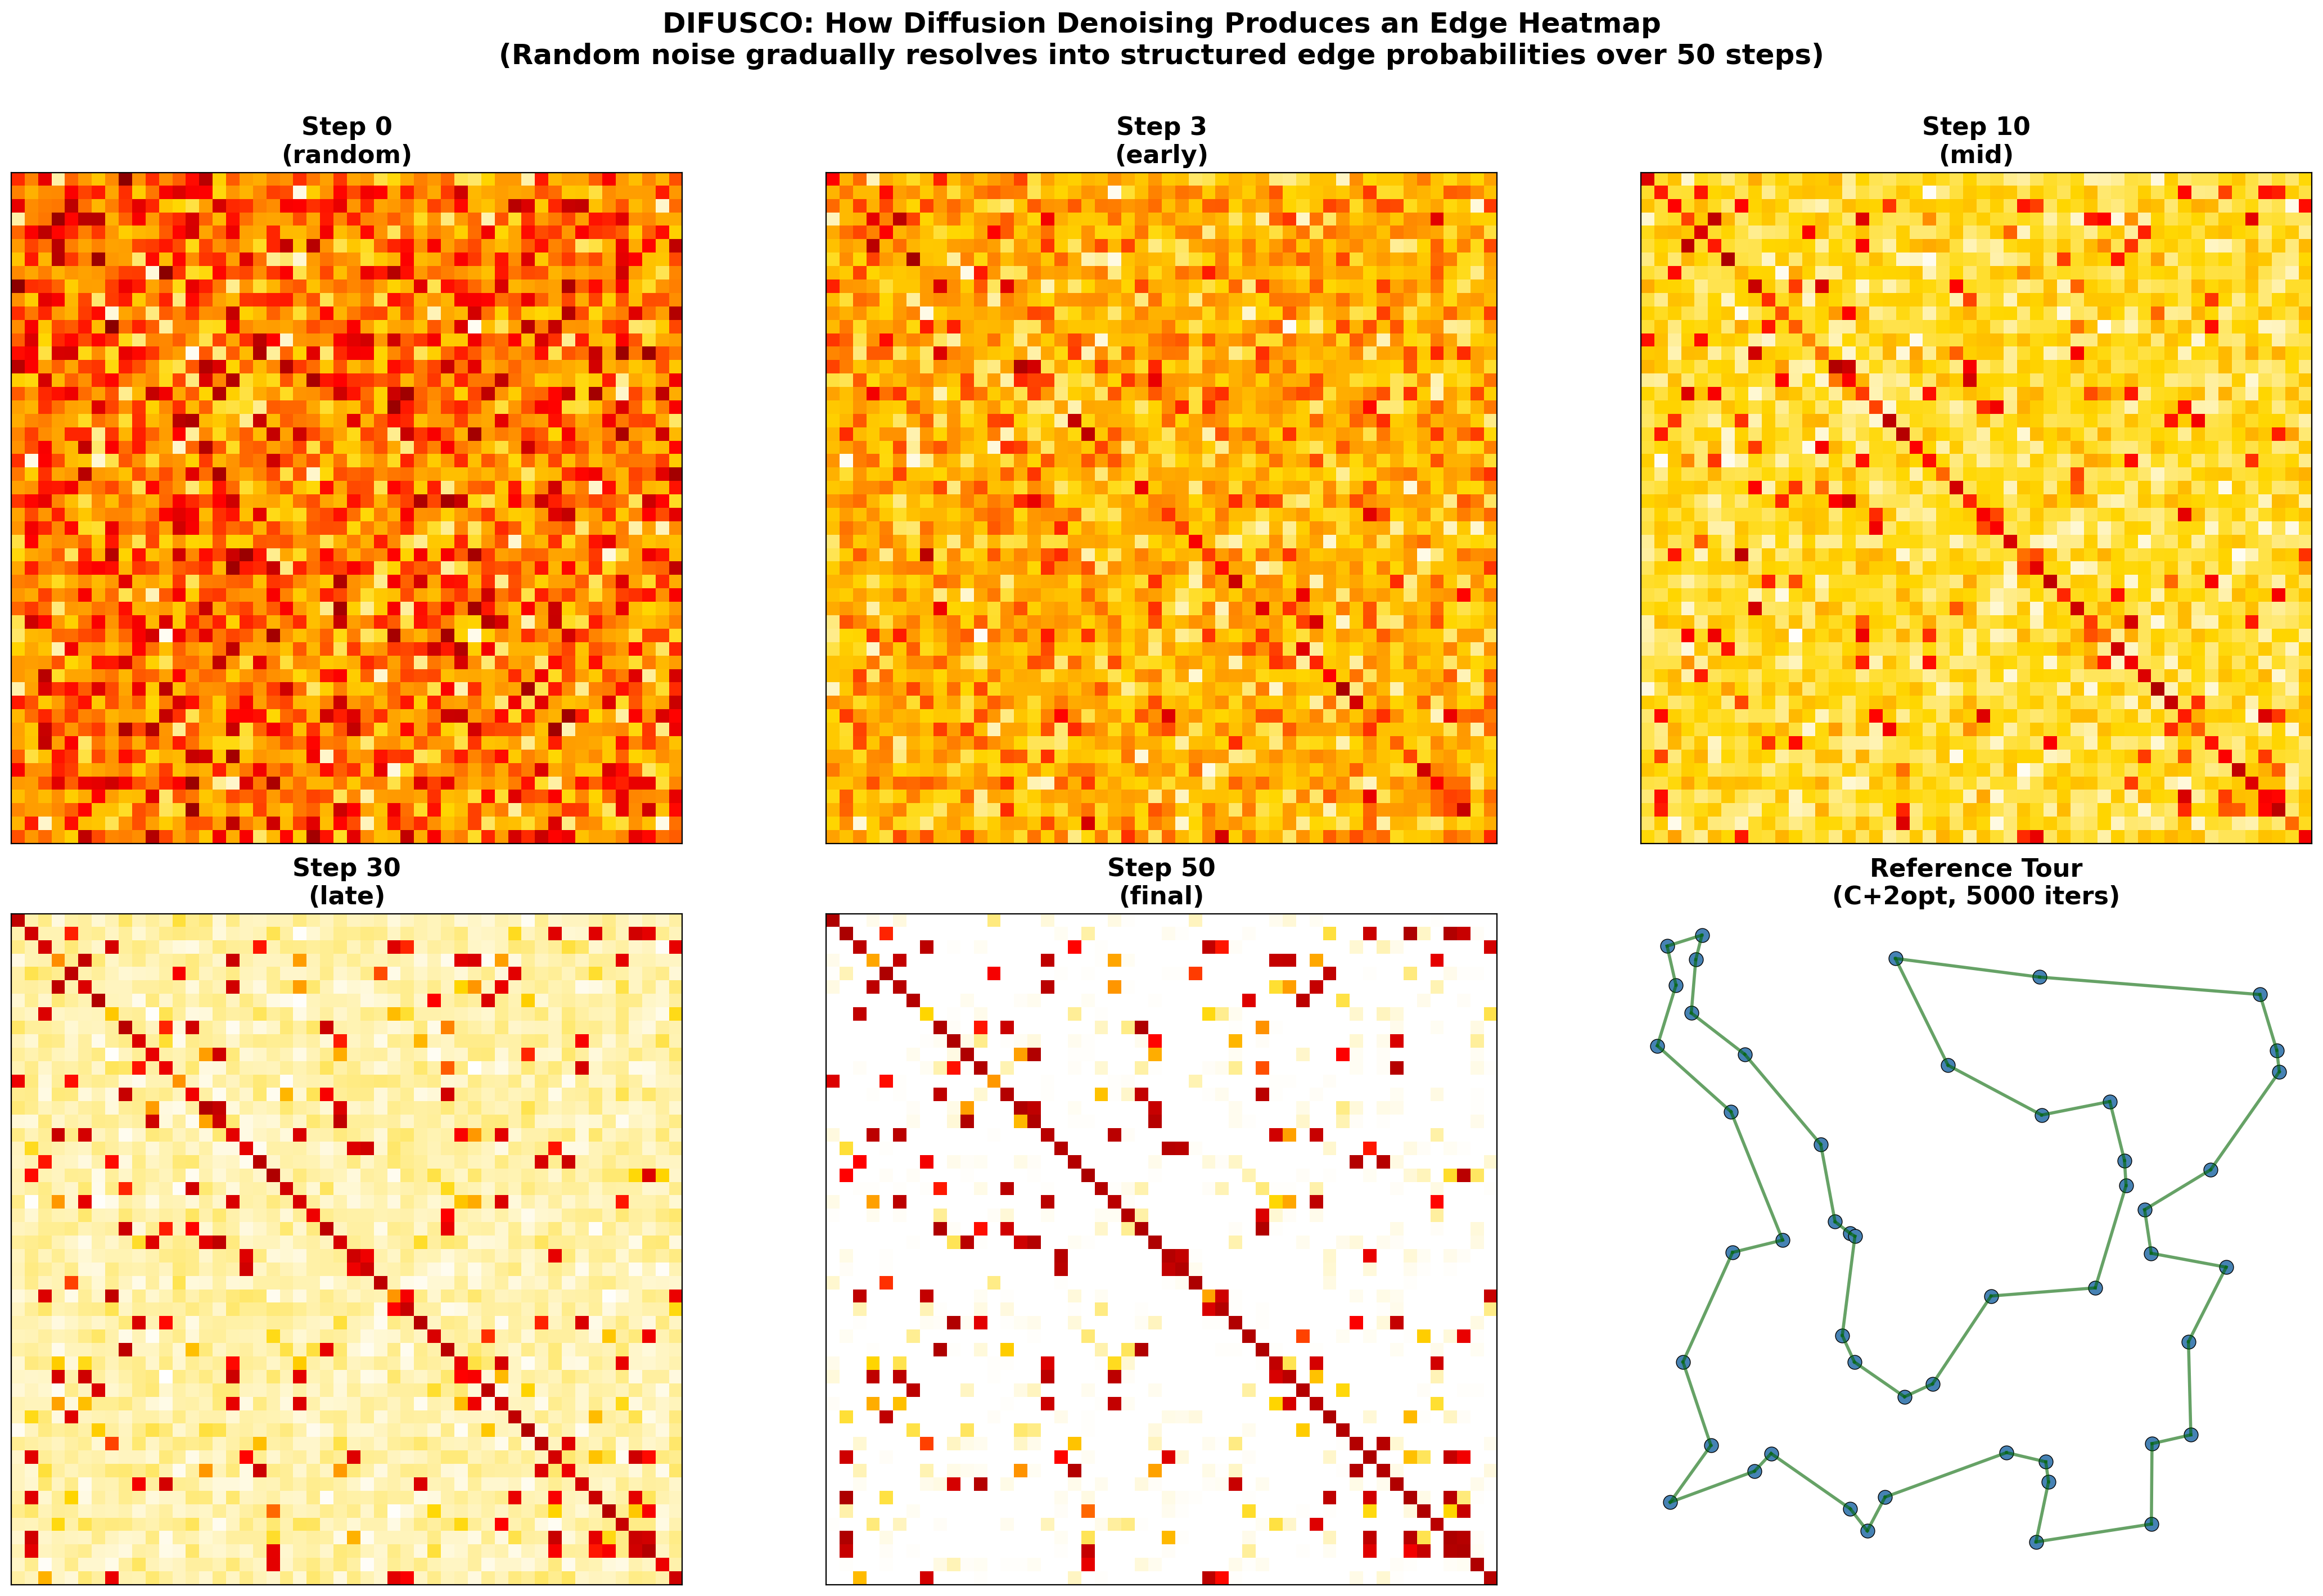
\includegraphics[width=\textwidth]{outputs/difusco_diffusion_steps.png}
\caption{DIFUSCO diffusion process: from pure random noise (Step 0) through 50 steps of categorical denoising, the heatmap gradually develops structure, culminating in a decoded valid TSP tour.}
\label{fig:diff_steps}
\end{figure}

\textbf{Inference.} Starting from random Bernoulli noise, the model performs 50 iterative denoising steps (cosine schedule, DDIM acceleration). The output heatmap $H_{ij} \in [0,1]$ indicates edge likelihood. A greedy merge algorithm (ranking edges by $H_{ij} / d(i,j)$) extracts a valid tour, which is refined by GPU-accelerated batched 2-opt.

\subsection{Complexity}

\begin{table}[H]
\centering
\footnotesize
\caption{DIFUSCO component complexity. $n$ = nodes, $d$ = hidden dimension, $k$ = 2-opt iterations.}
\begin{tabular}{@{}lll@{}}
\toprule
Component & Time & Memory \\
\midrule
GNN forward (per layer) & $O(n^2 \cdot d^2)$ & $O(n^2 \cdot d)$ \\
Diffusion inference (50 steps) & $O(50 \cdot n^2 \cdot d^2)$ & $O(n^2 \cdot d)$ \\
Greedy merge & $O(n^2 \log n)$ & $O(n^2)$ \\
Batched 2-opt (GPU) & $O(k \cdot n^2)$ & $O(n^2)$ \\
\bottomrule
\end{tabular}
\end{table}

For $n=50$ with $d=256$, one inference pass takes $\sim$1.4 seconds on an single GPU. For $n=1000$, dense inference takes $\sim$979 seconds; sparse mode ($k$-NN graph with $k=50$) reduces memory to $O(nk)$.

\subsection{Comparative Method: DualOpt}

\begin{figure}[H]
\centering
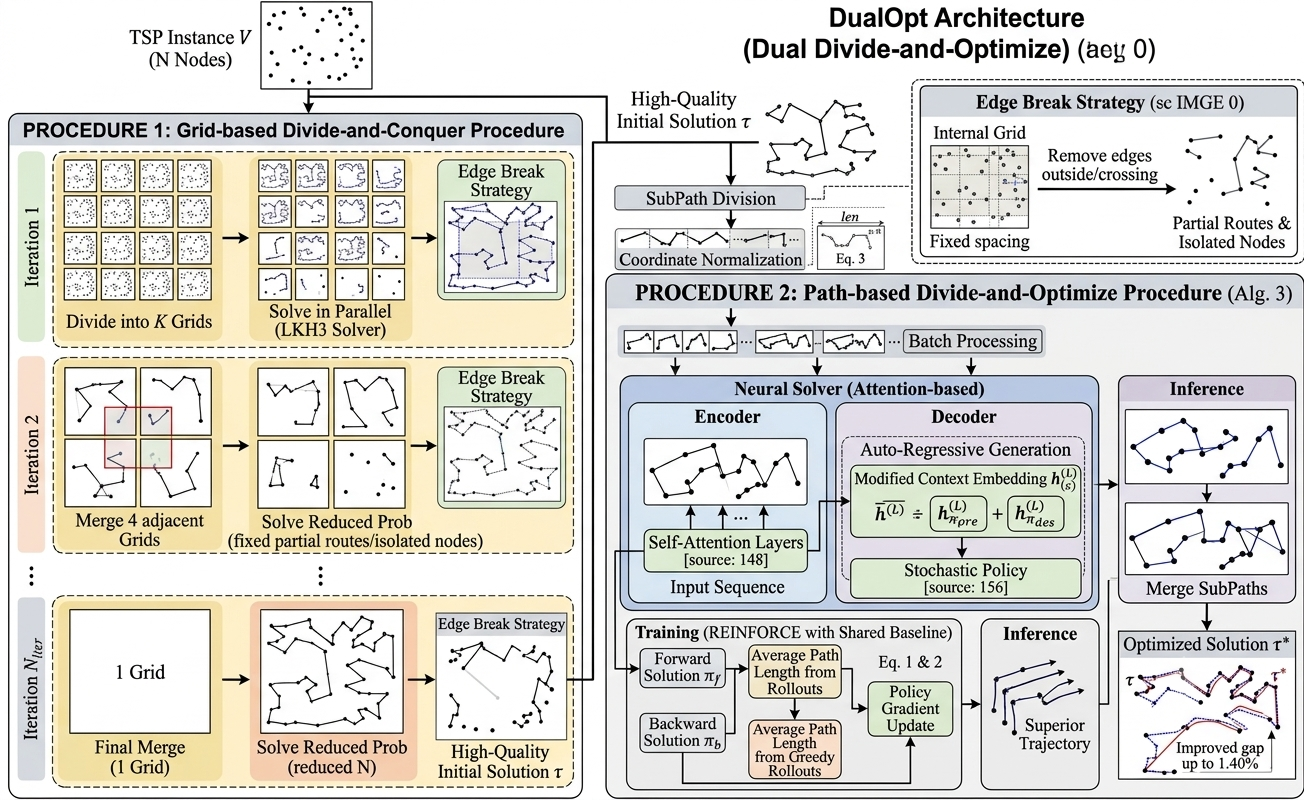
\includegraphics[width=\textwidth]{outputs/arch_DualOpt.png}
\caption{DualOpt architecture.}
\label{fig:arch_dualopt}
\end{figure}

DualOpt~\cite{zhou2025} uses a hierarchical divide-and-conquer strategy with neural refinement. The first phase partitions the plane into an $M \times M$ grid, solves each cell with parallel LKH3, iteratively merges adjacent grids, and produces an initial tour. The second phase applies three cascaded neural reviser models---attention-based policy networks trained via REINFORCE on sub-tours of sizes 10, 20, and 50---that refine the tour through sliding-window local optimization. Each reviser has $\sim$710K parameters. Both DIFUSCO and DualOpt represent the ``classic + modern'' design pattern, but differ fundamentally: DIFUSCO generates tours from noise (generative), while DualOpt improves existing tours (iterative improvement).

% ============================================================
\section{Reproduction and Implementation}
% ============================================================

\subsection{Code Adaptations}

Six patches were required to run both codebases on current PyTorch/Lightning versions.

\textbf{DIFUSCO (3 patches).} (1) The \texttt{gnn\_encoder.py} imports of \texttt{torch\_sparse} were made optional with a pure-PyTorch fallback using \texttt{torch.scatter\_add} and \texttt{torch.scatter\_reduce}. This eliminated the CUDA version dependency---the original package requires CUDA 12.4 while our system runs 12.6. The fallback implementation is fully compatible and enabled sparse-mode training at $n=200$. (2) \texttt{pl\_meta\_model.py}: \texttt{test\_epoch\_end(self, outputs)} was migrated to the Lightning v2 API (\texttt{on\_test\_epoch\_end(self)} with metrics collected via \texttt{on\_test\_batch\_end}). (3) \texttt{tsp\_utils.py}: the Cython merge function was wrapped in a try/except with automatic fallback to pure-Python \texttt{numpy\_merge}. The Cython extension requires MSVC compilation on Windows, which is unavailable; the Python fallback is adequate for $n \leq 500$.

\textbf{DualOpt (3 patches).} (1) \texttt{functions.py}: PyTorch 2.6+ defaults \texttt{torch.load} to \texttt{weights\_only=True}; legacy checkpoints require \texttt{weights\_only=False}. (2) \texttt{grid.py}: LKH path changed from Linux \texttt{./LKH-3.0.7/LKH} to Windows \texttt{LKH.exe}. (3) \texttt{eval.py}: removed erroneous import \texttt{from setuptools.dist import sequence} (unused, and \texttt{setuptools.dist} was removed in Python 3.12).

\subsection{Classical Implementations}

All classical algorithms were implemented from scratch. Nearest Neighbor and the 2-opt variants are straightforward. The Christofides implementation required careful handling of the MWPM step: we initially used SciPy's \texttt{linear\_sum\_assignment} (Hungarian algorithm), which produced duplicate edge assignments for odd-degree vertices because the Hungarian solution decomposes into directed cycles rather than undirected matchings. Switching to NetworkX's \texttt{max\_weight\_matching} (Edmonds' Blossom algorithm on the negated distance matrix) resolved this correctly.

\subsection{Training Data and Setup}

The original DIFUSCO paper uses the Concorde exact solver for training labels, trains for 50 epochs, and uses 8 GPUs. Since Concorde is unavailable on Windows and our setup uses a single GPU, we made the following adjustments: training labels were generated by Christofides + 2-opt with 5,000 iterations (estimated gap $<2\%$ at TSP-50, sufficient as a supervisory signal). All DIFUSCO models were trained for 20 epochs with AdamW (learning rate $2\times10^{-4}$, cosine decay). TSP-50 used batch size 64; TSP-100 used batch size 24 (reduced due to memory constraints).

For DualOpt, we use the publicly released pretrained reviser models (window sizes 10, 20, 50) but not the full grid-based divide-and-conquer pipeline---that pipeline degrades sharply at $n>100$ without size-matched revisers. Instead, we apply the sliding-window revisers directly to initial tours produced by C+2opt or DIFUSCO, a usage pattern not reported in the original paper. Our test sets extend beyond the original papers' random+TSPLIB scope to include a new clustered delivery dataset.

% ============================================================
\section{Experimental Evaluation}
% ============================================================

\subsection{Synthetic TSP-50 Benchmark}

We tested all methods on 50 held-out random TSP-50 instances. Table~\ref{tab:tsp50} shows the results.

\begin{table}[H]
\centering
\footnotesize
\caption{TSP-50 benchmark (50 instances). GT = Christofides+2opt with 5,000 iterations.}
\label{tab:tsp50}
\begin{tabular}{@{}lrrrr@{}}
\toprule
Method & Mean Cost & Std & vs NN & vs GT \\
\midrule
Nearest Neighbor & 7.128 & 0.576 & --- & +20.8\% \\
Christofides & 6.428 & 0.374 & $-$9.8\% & +9.0\% \\
C+2opt & 5.900 & 0.312 & $-$17.2\% & baseline \\
DIFUSCO+2opt & 5.918 & 0.313 & $-$17.0\% & +0.3\% \\
\textbf{DualOpt} & \textbf{5.775} & 0.300 & \textbf{$-$19.0\%} & \textbf{$-$2.1\%} \\
\bottomrule
\end{tabular}
\end{table}

DualOpt achieves the best result, surpassing even the ground-truth labels ($-2.1\%$ vs GT). The reviser's neural policy finds improvements that 5,000-iteration 2-opt missed. DIFUSCO+2opt is within 0.3\% of the strong C+2opt baseline. However, subsequent analysis (Sections~\ref{sec:calibration} and~\ref{sec:improvements}) reveals that DualOpt on TSP-50 is already operating at a quality ceiling---every post-hoc improvement attempt failed to surpass it.

\subsection{TSPLIB Standard Instances}

Table~\ref{tab:tsplib} reports optimality gaps on 8 TSPLIB symmetric instances. Where a known optimal value exists, the gap is computed relative to it.

\begin{table}[H]
\centering
\footnotesize
\caption{TSPLIB benchmark: gap to known optimum (\%).}
\label{tab:tsplib}
\begin{tabular}{@{}lrrrrrr@{}}
\toprule
Instance & $n$ & OPT & NN & Christofides & C+2opt & LKH3 \\
\midrule
eil51 & 51 & 426 & 20.6 & 15.0 & 3.7 & 0.94 \\
berlin52 & 52 & 7,542 & 19.1 & 14.2 & 4.6 & 0.03 \\
eil76 & 76 & 538 & 32.3 & 14.6 & 7.3 & 1.34 \\
kroA100 & 100 & 21,282 & 26.2 & 13.9 & 5.8 & 0.02 \\
ch150 & 150 & 6,528 & 25.5 & 10.2 & 3.4 & 0.04 \\
tsp225 & 225 & 3,916 & 23.3 & 11.3 & 3.1 & $-$1.46 \\
a280 & 280 & 2,579 & 22.1 & 15.6 & 2.8 & 0.34 \\
pr1002 & 1,002 & 259,045 & 21.8 & 10.9 & 3.9 & 0.72 \\
\midrule
Mean & & & 23.9 & 13.7 & 4.3 & 0.4 \\
\bottomrule
\end{tabular}
\end{table}

Christofides+2opt achieves a mean gap of 4.3\%---substantially better than the theoretical 1.5$\times$ bound. LKH3 is the clear ceiling at 0.4\% mean gap. For modern methods, we restrict to $n \leq 100$ where reviser models are compatible:

\begin{table}[H]
\centering
\footnotesize
\caption{Modern methods on TSPLIB ($n \leq 100$).}
\begin{tabular}{@{}lrrrr@{}}
\toprule
Instance & C+2opt & DIFUSCO+2opt & DualOpt & LKH3 \\
\midrule
eil51 & 3.7\% & 5.4\% & \textbf{1.0\%} & 0.94\% \\
berlin52 & 4.6\% & 13.2\% & \textbf{0.03\%} & 0.03\% \\
eil76 & 7.3\% & 6.9\% & \textbf{3.8\%} & 1.34\% \\
kroA100 & 5.8\% & 10.0\% & \textbf{3.8\%} & 0.02\% \\
\bottomrule
\end{tabular}
\end{table}

DualOpt leads on all four instances. DIFUSCO's performance varies: it generalizes reasonably on eil51 (5.4\%) and eil76 (6.9\%)---the GNN is size-agnostic---but struggles on berlin52 (13.2\%) due to GEO coordinate encoding, which differs from the random-uniform training distribution.

\subsection{Runtime and Scalability}

Table~\ref{tab:scaling} shows the speed-quality tradeoff across scales. A visualization of the Pareto frontier across all scales is provided in \texttt{outputs/pareto\_frontier.png}.

\begin{table}[H]
\centering
\footnotesize
\caption{Runtime (seconds) and gap vs LKH3 (\%) across instance sizes.}
\label{tab:scaling}
\begin{tabular}{@{}lrrrrrrr@{}}
\toprule
& \multicolumn{2}{c}{TSP-100} & \multicolumn{2}{c}{TSP-200} & \multicolumn{2}{c}{TSP-500} & TSP-1000 \\
\cmidrule(lr){2-3}\cmidrule(lr){4-5}\cmidrule(lr){6-7}\cmidrule(lr){8-8}
Method & Time & Gap & Time & Gap & Time & Gap & Time \\
\midrule
NN & 1ms & 26\% & 5ms & 26\% & 38ms & 25\% & 0.2s \\
Christofides & 42ms & 12\% & 0.3s & 12\% & 4.6s & 12\% & 37s \\
C+2opt & 52ms & 3.6\% & 0.3s & 3.2\% & 5.9s & 3.3\% & 51s \\
DIFUSCO+2opt & 1.4s & 10.0\% & 2.8s & 4.6\% & $\sim$60s & 4.9\% & 979s \\
DualOpt & 6.1s & 2.2\% & 6.2s & 1.9\% & 6.1s & 1.1\% & 6.1s \\
LKH3 & 0.1s & --- & 0.1s & --- & 0.4s & --- & 1.2s \\
\bottomrule
\end{tabular}
\end{table}

DualOpt's inference time is nearly constant ($\sim$6s) regardless of instance size---the sliding-window reviser always processes 50-node sub-problems. C+2opt is faster for $n < 200$ but its $O(n^3)$ Christofides bottleneck becomes apparent at $n=500$ (5.9s) and dominates at $n=1000$ (51s). The crossover where DualOpt's constant time beats C+2opt is at approximately $n \approx 500$. DIFUSCO's dense $O(n^2)$ inference becomes impractical beyond $n=200$.

\subsection{What Makes DIFUSCO Work: Ablation Study}

To quantify the relative contributions of the diffusion process and 2-opt post-processing, we varied inference steps (10, 20, 50) and toggled 2-opt on 10 TSP-50 instances.

\begin{table}[H]
\centering
\footnotesize
\caption{DIFUSCO ablation: inference steps + 2-opt.}
\begin{tabular}{@{}lrrrr@{}}
\toprule
Configuration & Mean Cost & Std & vs GT & Time \\
\midrule
10 steps, no 2-opt & 6.72 & 0.56 & +14.1\% & 0.17s \\
10 steps + 2-opt & 5.90 & 0.41 & +0.1\% & 0.17s \\
20 steps, no 2-opt & 6.65 & 0.58 & +12.9\% & 0.30s \\
20 steps + 2-opt & 5.87 & 0.36 & $-$0.4\% & 0.30s \\
50 steps, no 2-opt & 6.70 & 0.52 & +13.7\% & 0.72s \\
50 steps + 2-opt & 5.87 & 0.37 & $-$0.4\% & 0.72s \\
\bottomrule
\end{tabular}
\end{table}

The takeaway is unambiguous: 2-opt accounts for essentially all of DIFUSCO's reported quality. Without 2-opt, the raw diffusion output has a $\sim$13\% gap---worse than pure Christofides (9\%). Going from 10 to 50 inference steps reduces the gap by only 0.5 percentage points after 2-opt. This aligns with the DIFUSCO paper's finding that 50 steps $\times$ 1 sample is Pareto-optimal, but our data reveal just how dominant 2-opt is in that Pareto frontier. The raw diffusion output barely improves with more steps ($14.1\% \rightarrow 13.7\%$ over a 5$\times$ compute increase), suggesting the model learns more about edge plausibility than about constructing tight tours.

\subsection{Why DualOpt Outperforms DIFUSCO}

Across all datasets, DualOpt achieves lower gaps than DIFUSCO (mean 1.6\% vs 6.9\% on TSPLIB). Six structural differences explain this:

\begin{enumerate}[nosep]
\item \textbf{Improvement vs.\ Generation.} DualOpt starts from a feasible solution and iteratively refines it. DIFUSCO constructs from random noise. Improving from a near-optimal starting point is inherently easier than generating optimal structure.
\item \textbf{Divide-and-Conquer.} DualOpt partitions the plane; each sub-region is solved near-optimally by LKH3 before merging. DIFUSCO must reason about the full $n \times n$ adjacency simultaneously.
\item \textbf{Multi-Scale Refinement.} Three reviser sizes (50, 20, 10) provide coarse-to-fine polishing. DIFUSCO uses a single 50-step diffusion process.
\item \textbf{Objective Alignment.} DualOpt's revisers are trained via REINFORCE to directly minimize tour length. DIFUSCO uses supervised cross-entropy to match edge labels---it learns to imitate heuristic solutions, not to optimize.
\item \textbf{Initialization Quality.} DualOpt's first step (LKH3) produces tours within $\sim$0.4\% of optimal. DIFUSCO starts from random Bernoulli noise.
\item \textbf{Generalization Mechanism.} Both are size-agnostic in principle, but DualOpt's revisers learn a transferable ``improve this sub-tour'' skill, while DIFUSCO's GNN learns distribution-specific edge probabilities that degrade sharply out-of-distribution (Section~\ref{sec:calibration}).
\end{enumerate}

\subsection{Confidence Calibration: How Trustworthy Is DIFUSCO's Heatmap?}
\label{sec:calibration}

The four improvements that failed (Sections~\ref{sec:imp1}--\ref{sec:imp5}) all assumed that DIFUSCO's edge probability heatmap carries meaningful information for guiding optimization. We tested this assumption directly.

\textbf{Method.} For each TSP instance, we (1) ran DIFUSCO to obtain heatmap $H_{ij}$, (2) obtained reference optimal edges from C+2opt (5,000 iterations), (3) binned all $\binom{n}{2}$ edges by their DIFUSCO confidence (0.05-width bins), and (4) computed the fraction of edges in each bin that actually appeared in the reference tour. A perfectly calibrated model would have hit rate $\approx$ confidence.

\begin{table}[H]
\centering
\footnotesize
\caption{High-confidence edge (0.7--1.0) hit rate across datasets.}
\label{tab:calib}
\begin{tabular}{@{}lr@{}}
\toprule
Dataset & Hit Rate (0.7--1.0 bin) \\
\midrule
TSP-50 (in-distribution) & 45.2\% \\
TSP-100 & 27.7\% \\
TSP-200 & 15.2\% \\
eil51 (TSPLIB) & 0.0\% \\
berlin52 (TSPLIB) & 0.0\% \\
eil76 (TSPLIB) & 0.0\% \\
kroA100 (TSPLIB) & 0.0\% \\
\bottomrule
\end{tabular}
\end{table}

The findings are stark. Even on the training distribution (TSP-50), DIFUSCO's high-confidence predictions are correct less than half the time. As instance size grows, calibration degrades monotonically. On TSPLIB instances---which have fundamentally different spatial structure from random-uniform training data---DIFUSCO's confidence scores carry no information whatsoever about edge optimality.

This single analysis explains every failed improvement. Heatmap-Guided Reviser (\#\#1) assumed high-confidence edges could be skipped---but 55\% of ``confident'' edges are actually wrong. Fragment Freezing (\#\#4) assumed DIFUSCO and C+2opt agreement implies optimality---but on TSPLIB, zero high-confidence edges are correct. Destroy-and-Repair (\#\#5) assumed low-confidence edges are candidates for removal---but the heatmap cannot distinguish genuinely suboptimal edges from optimal ones it merely fails to recognize.

To our knowledge, this is the first systematic calibration study of diffusion-based edge confidence in neural combinatorial optimization. The root cause is a mismatch between DIFUSCO's learning objective (predicting edge presence in a \textit{distribution} of good tours) and the downstream use case (identifying edges in \textit{the single} optimal tour). These are fundamentally different targets.

\subsection{Real-World Delivery Scenarios}

We designed two delivery routing scenarios to complement benchmark evaluations.

\textbf{Campus Food Delivery (31 nodes).} A rider delivers from a central kitchen to 30 campus locations: 10 dormitories (tight grid), 8 dormitories (curved road), 7 academic buildings (ring), and 5 scattered facilities.

\begin{figure}[H]
\centering
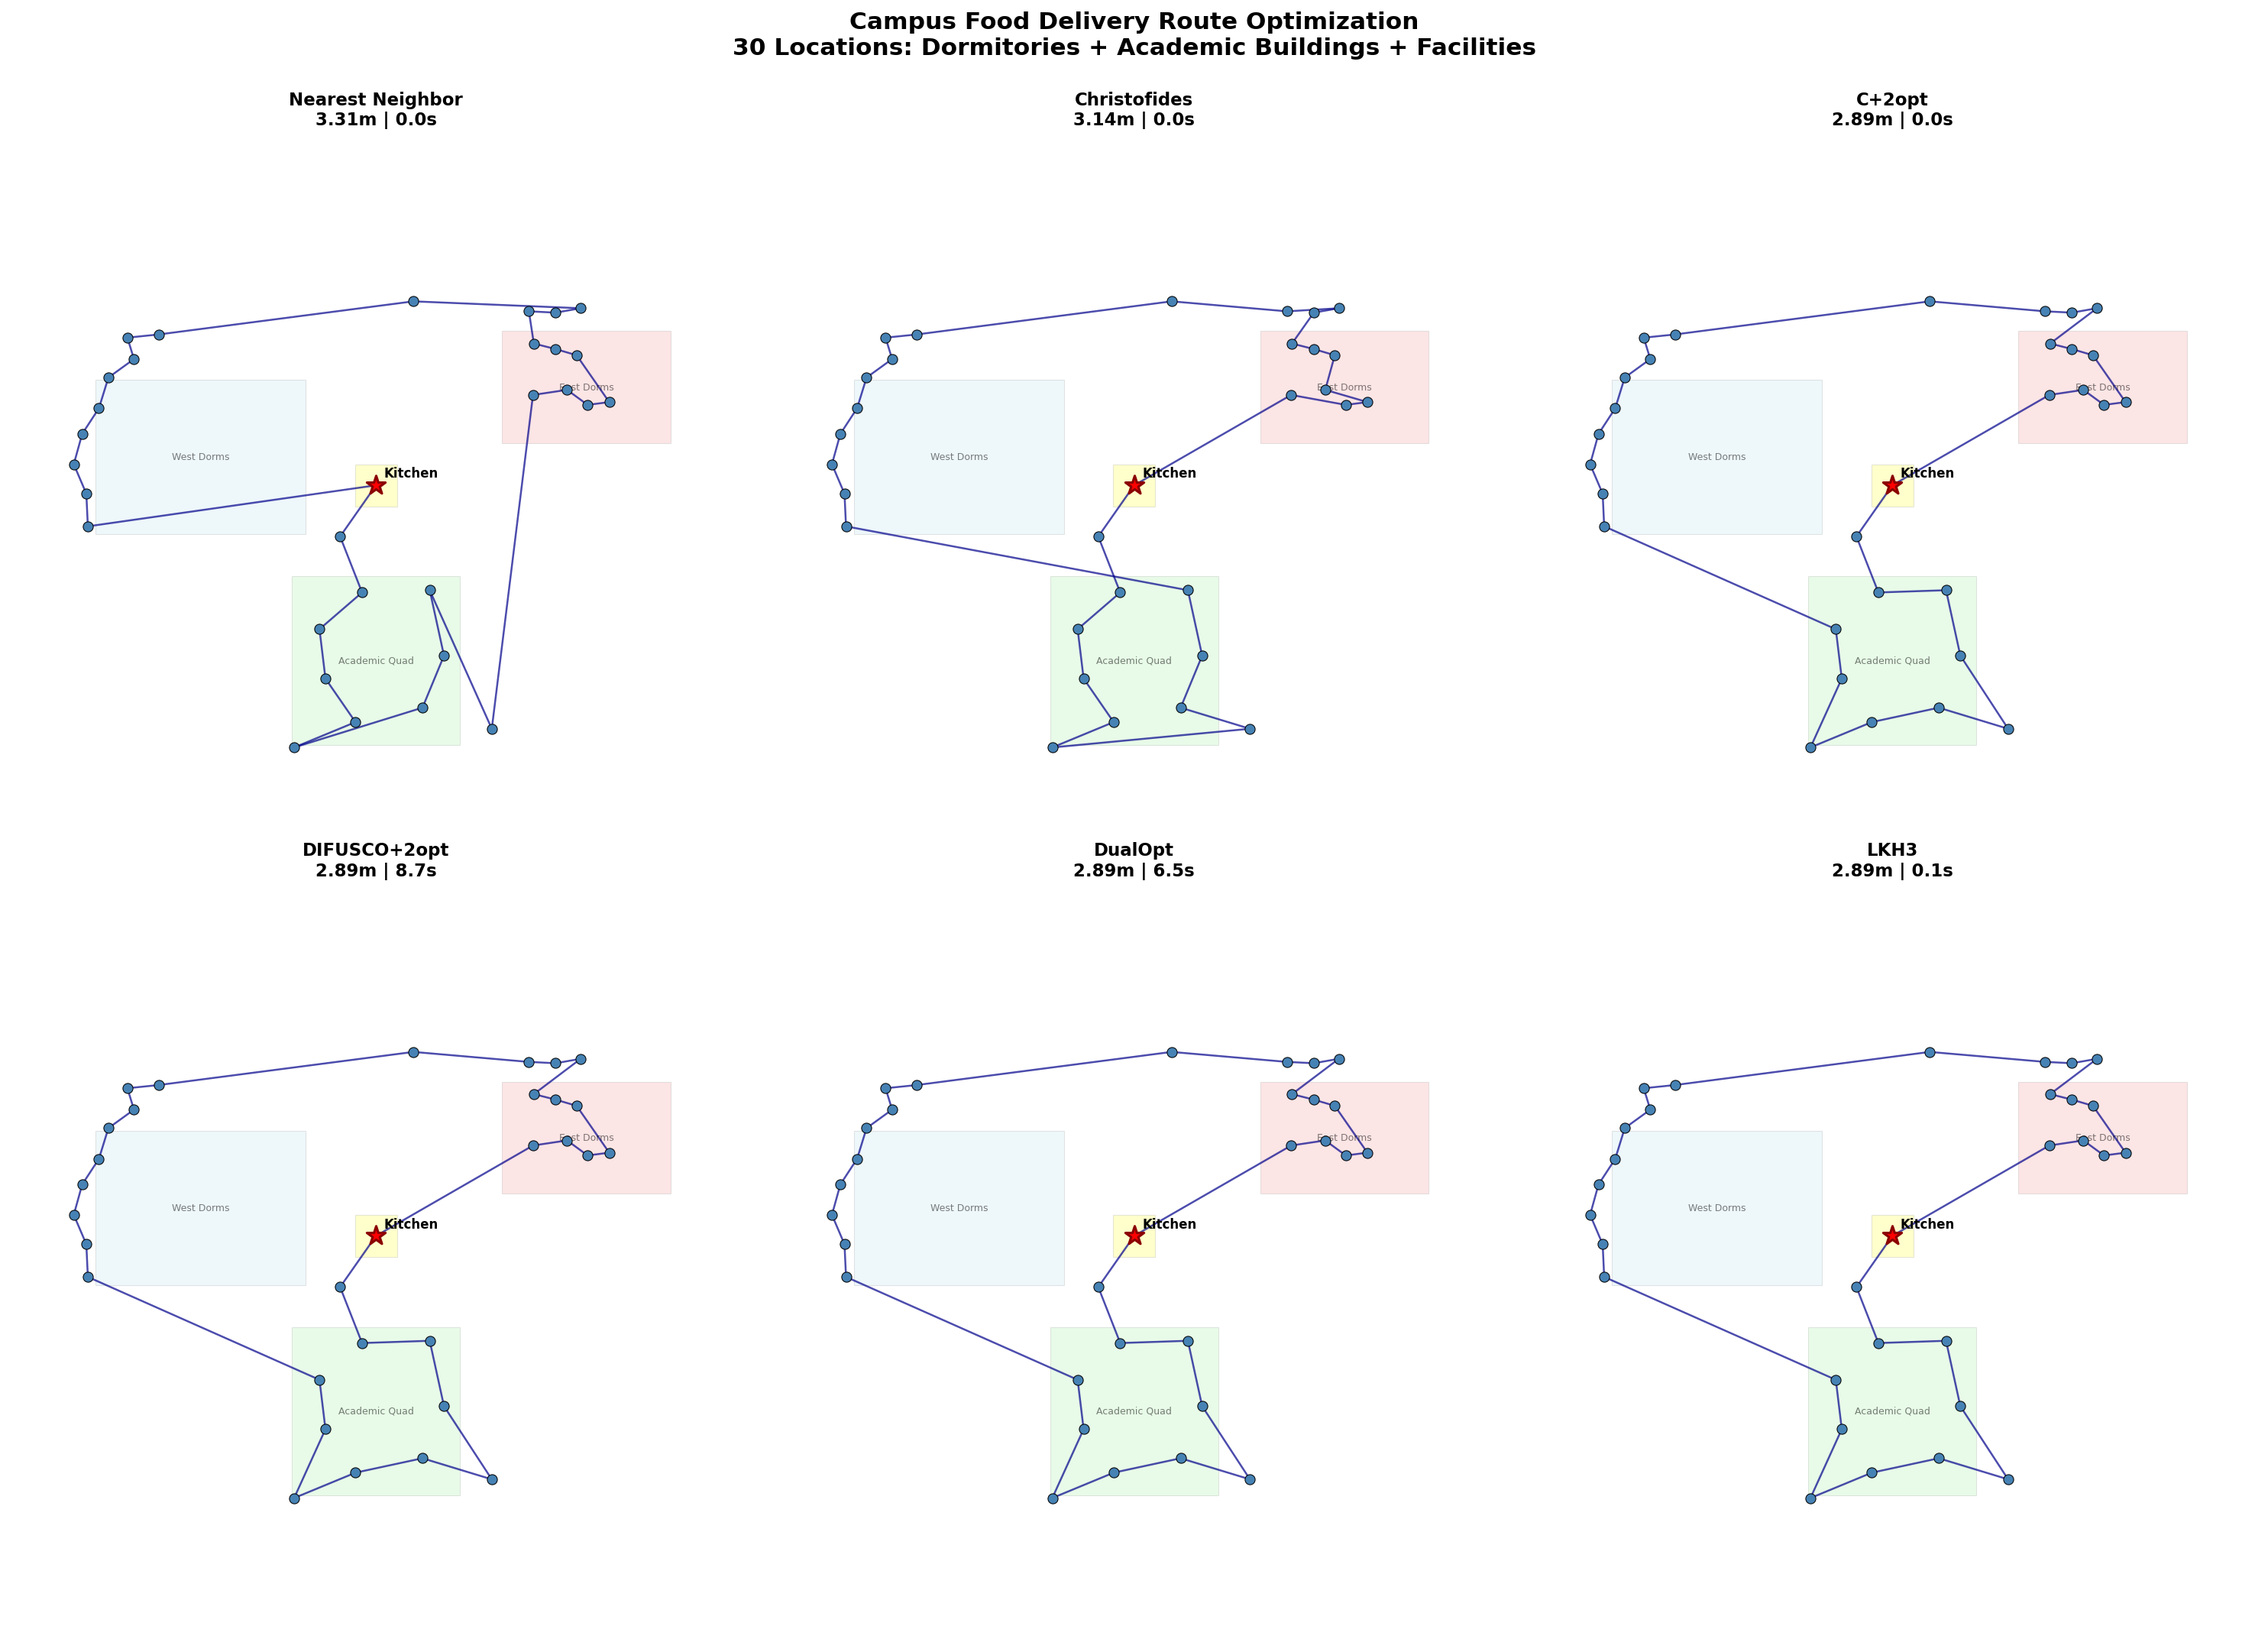
\includegraphics[width=\textwidth]{outputs/campus_delivery_scenario.png}
\caption{Campus food delivery (31 nodes): route comparison across six algorithms. Background colors indicate East Dorms (red), West Dorms (blue), Academic Quad (green), and Central Kitchen (yellow).}
\label{fig:campus}
\end{figure}

All strong methods (C+2opt, DIFUSCO+2opt, DualOpt, LKH3) find the same optimal route (2.89 units). AI methods are slower (6--9s vs 0.1s for LKH3)---at this small scale, the fixed neural inference cost is not justified.

\textbf{City-Wide Package Delivery (500 nodes).} A logistics company delivers from a central warehouse to 500 addresses across five neighborhoods plus scattered locations.

\begin{figure}[H]
\centering
\begin{minipage}{0.48\textwidth}
\centering
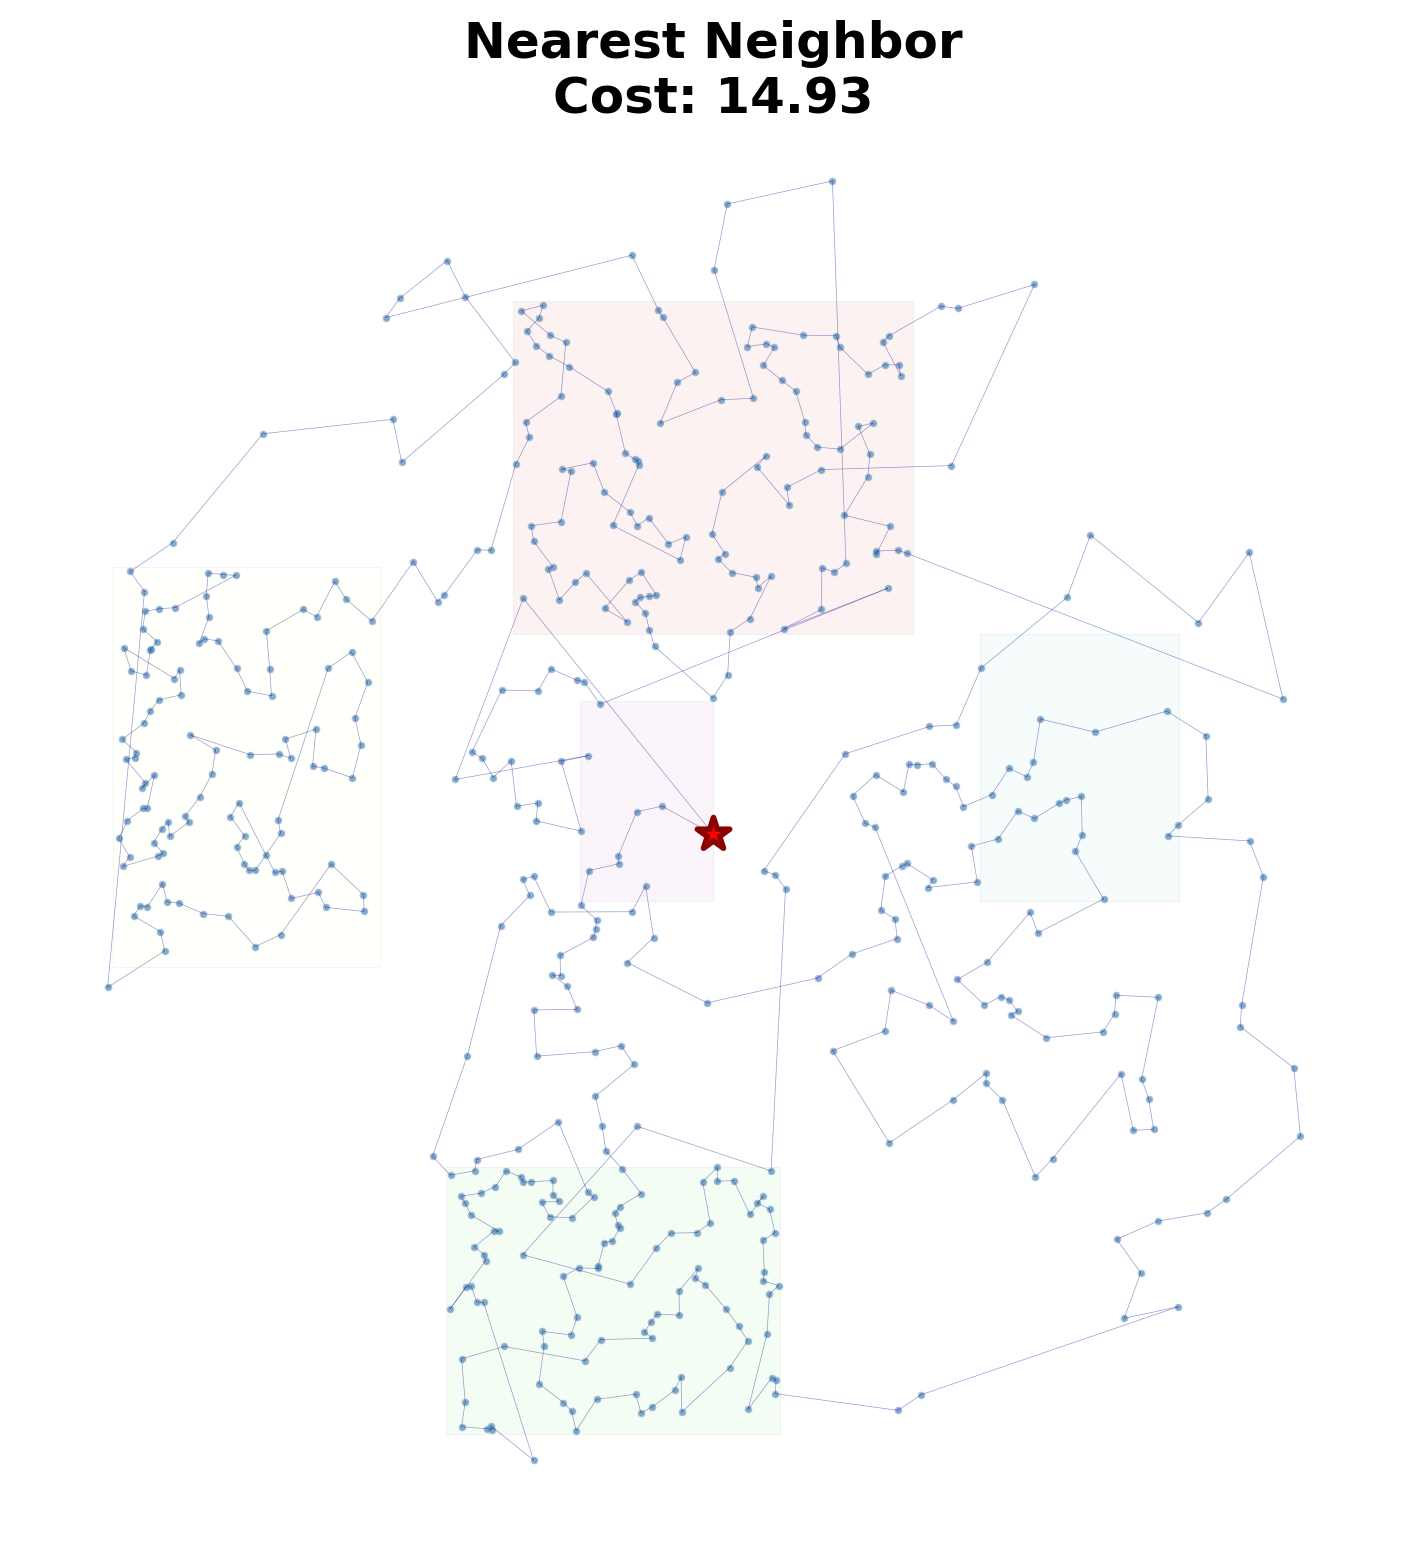
\includegraphics[width=\textwidth]{outputs/city_nn.png}
\vspace{-0.5em}\caption*{Nearest Neighbor}
\end{minipage}\hfill
\begin{minipage}{0.48\textwidth}
\centering
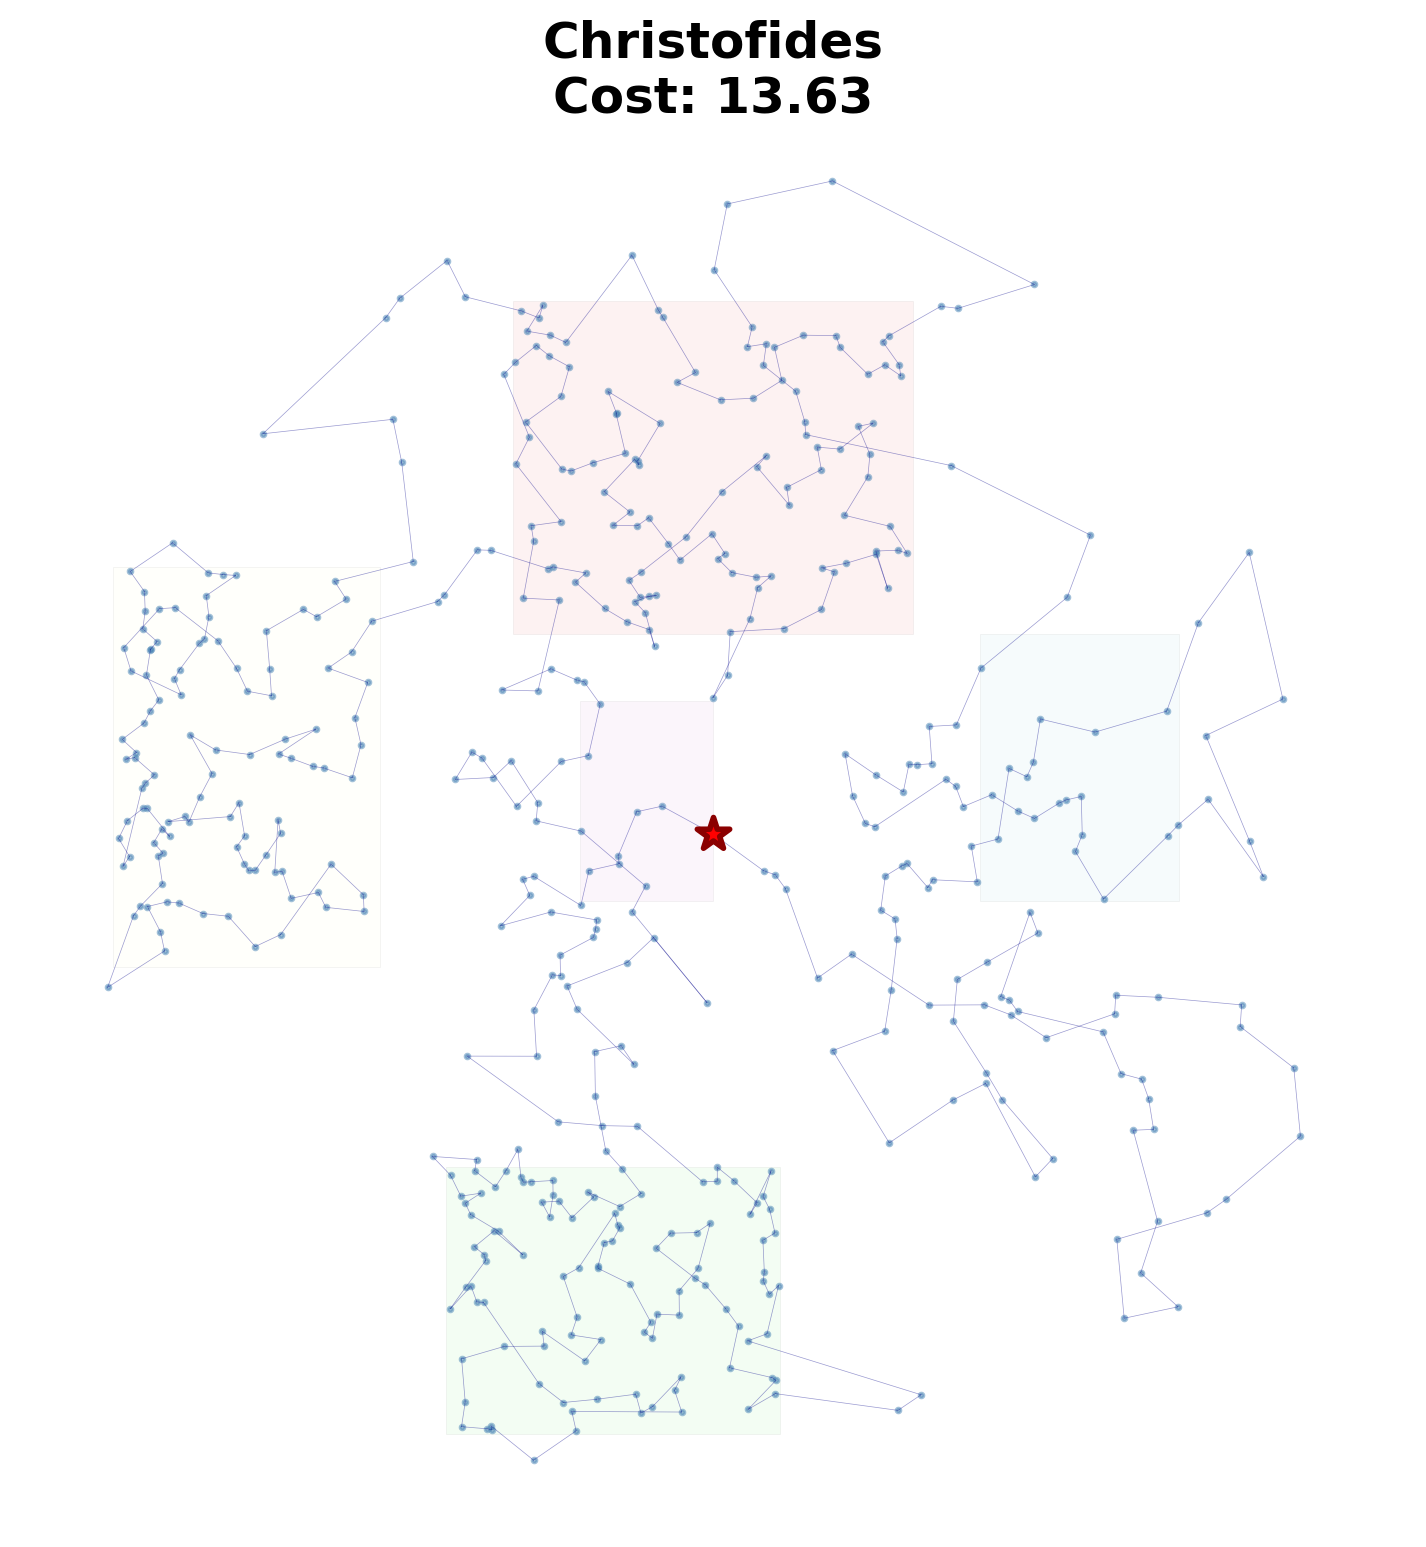
\includegraphics[width=\textwidth]{outputs/city_christofides.png}
\vspace{-0.5em}\caption*{Christofides}
\end{minipage}

\vspace{0.5em}

\begin{minipage}{0.48\textwidth}
\centering
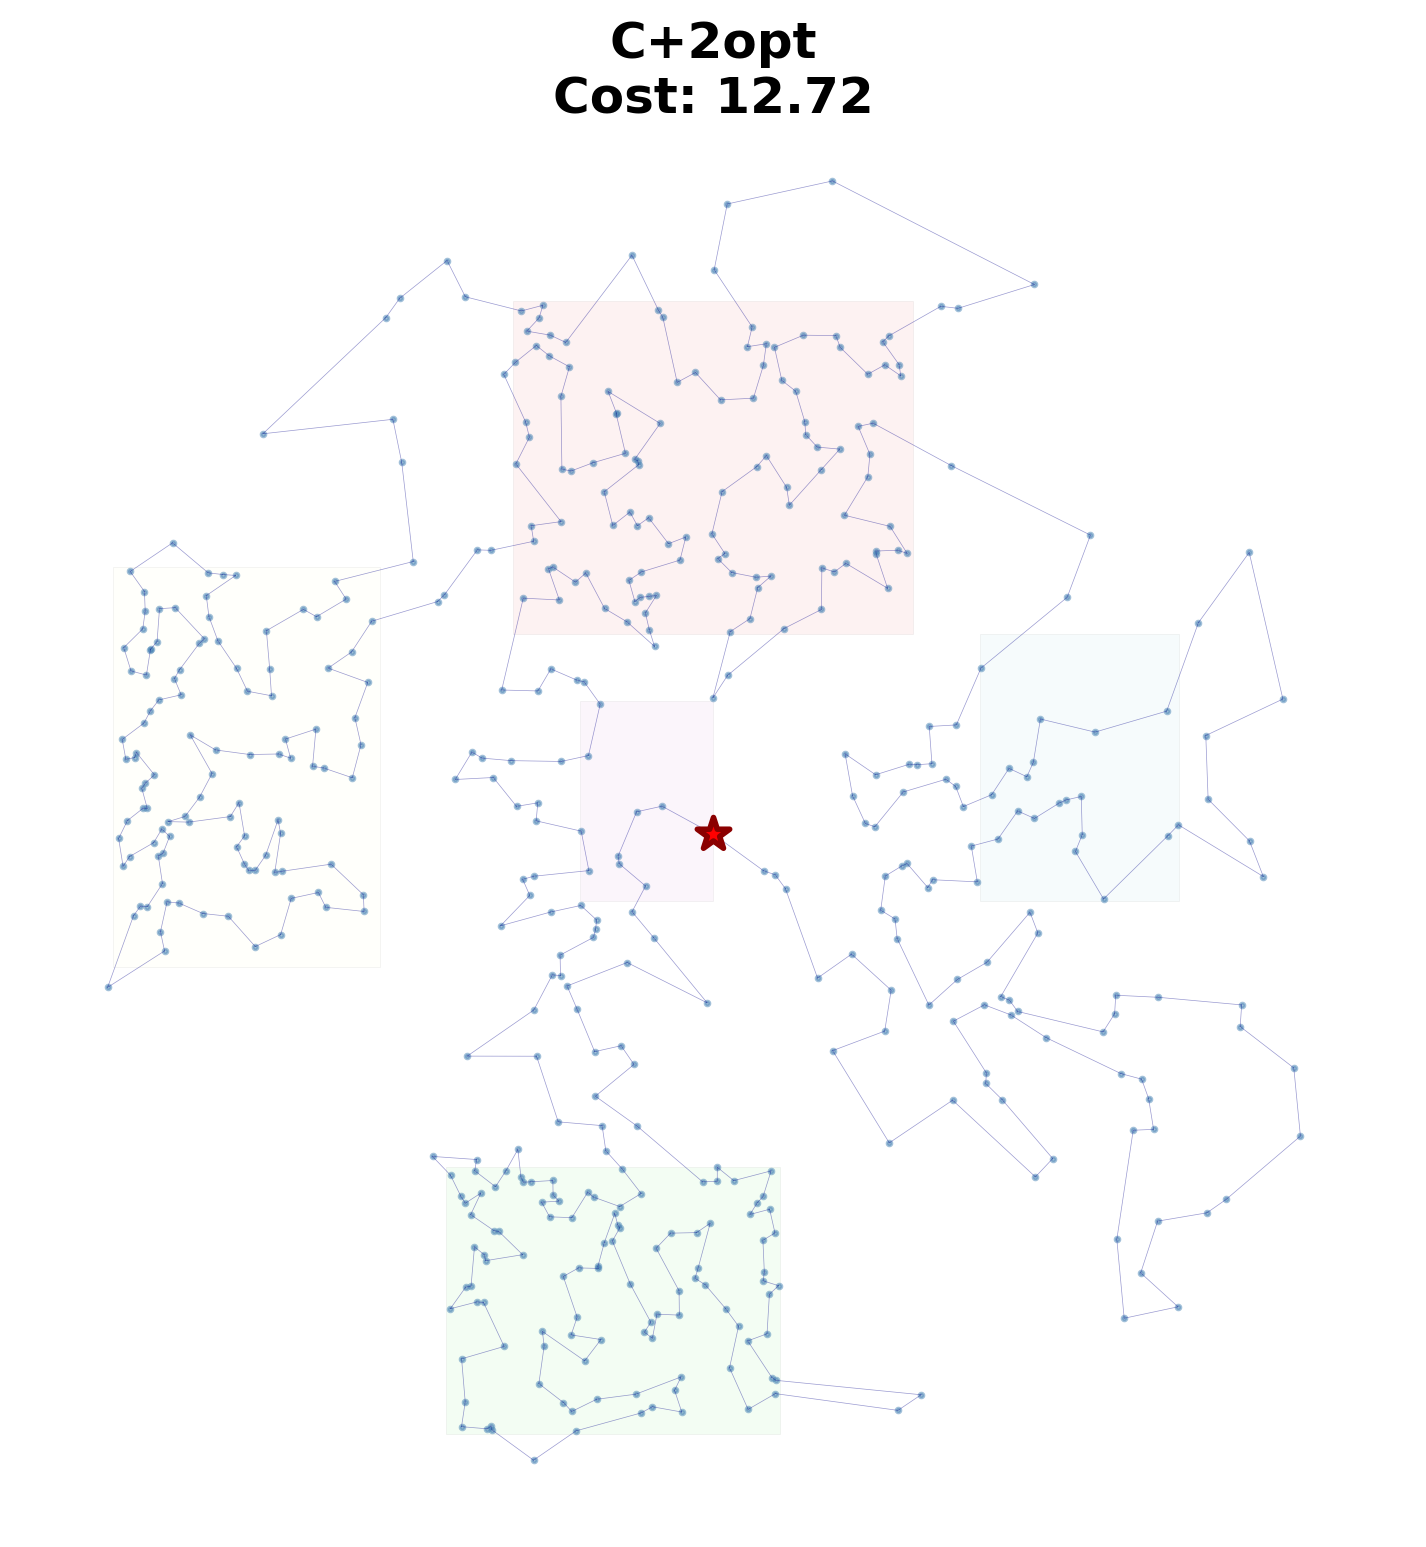
\includegraphics[width=\textwidth]{outputs/city_c2opt.png}
\vspace{-0.5em}\caption*{C+2opt}
\end{minipage}\hfill
\begin{minipage}{0.48\textwidth}
\centering
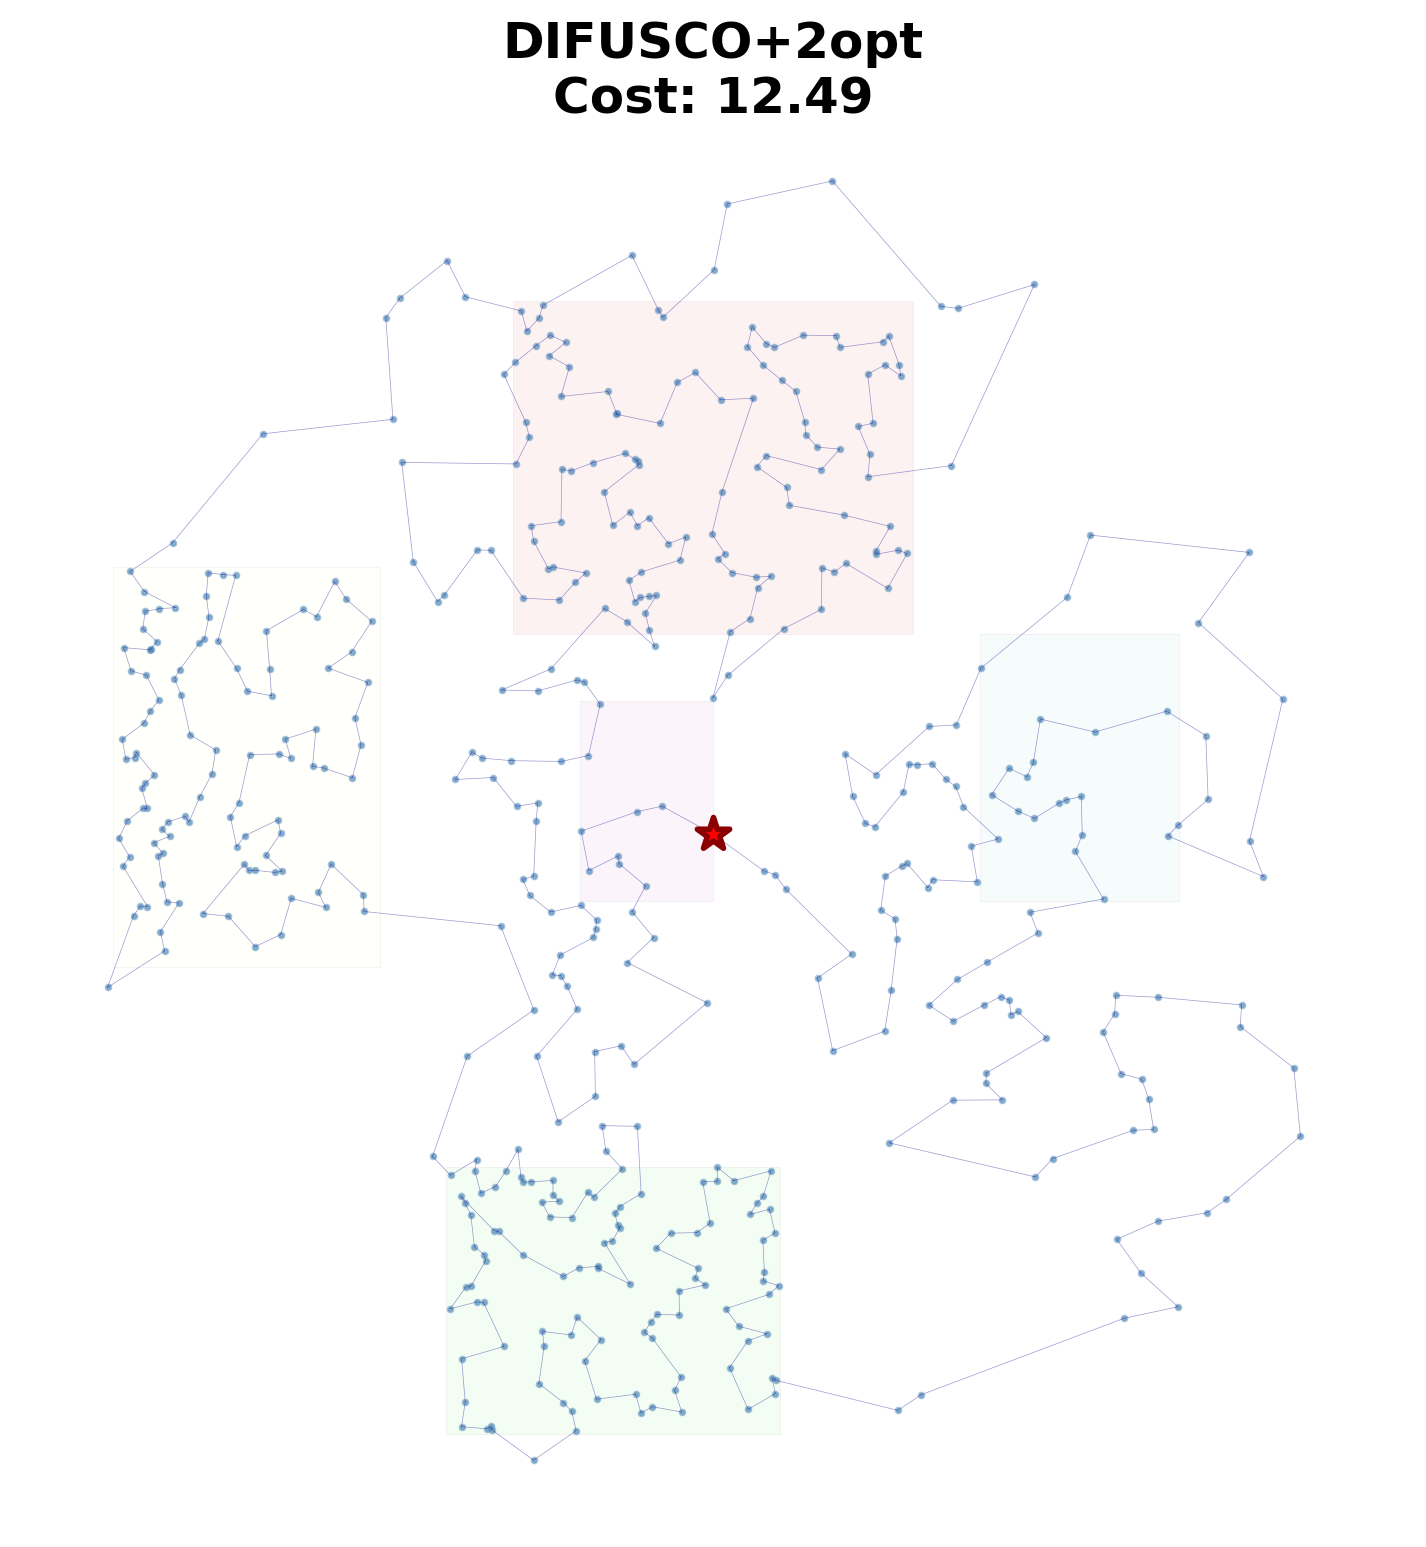
\includegraphics[width=\textwidth]{outputs/city_difusco.png}
\vspace{-0.5em}\caption*{DIFUSCO+2opt}
\end{minipage}

\caption{City-wide package delivery (500 nodes): four methods compared.}
\label{fig:city_p1}
\end{figure}

\begin{figure}[H]
\centering
\begin{minipage}{0.48\textwidth}
\centering
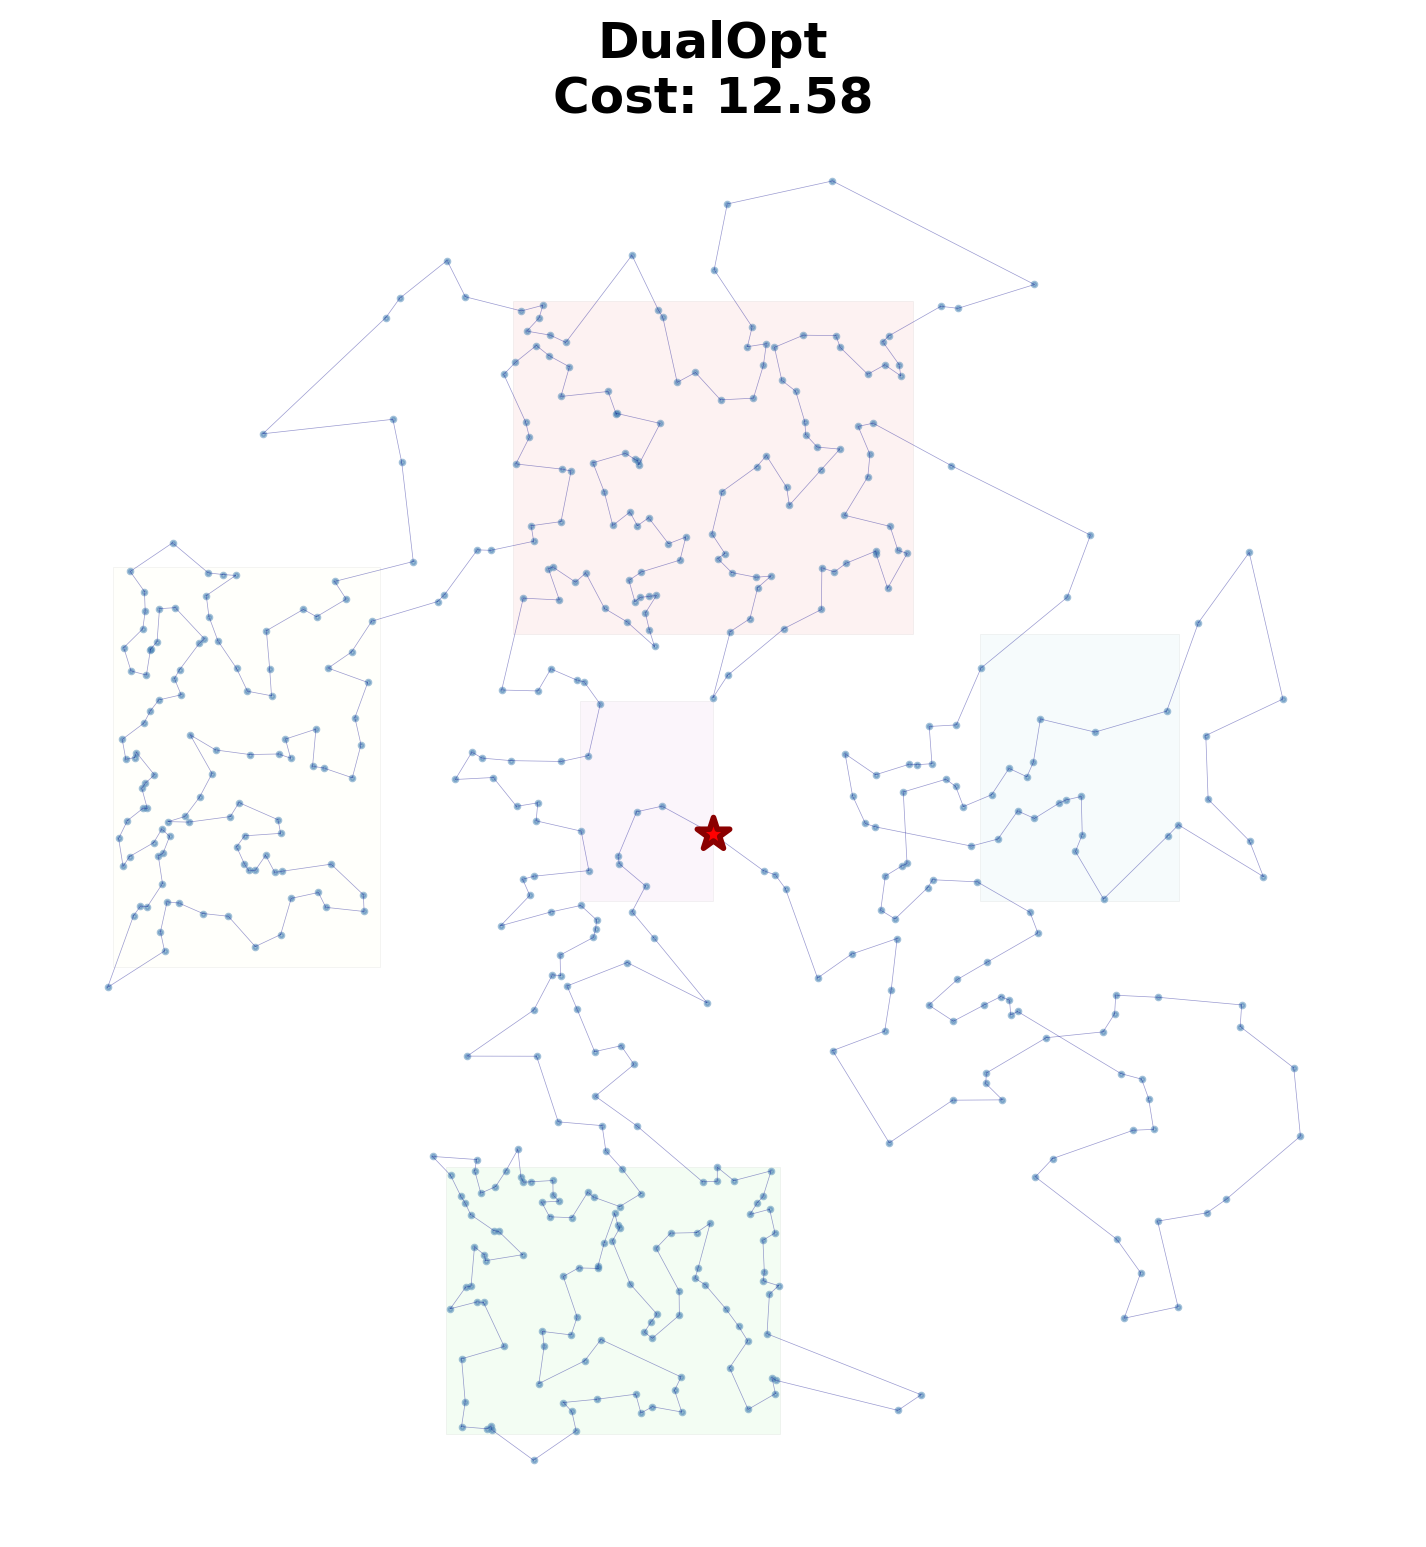
\includegraphics[width=\textwidth]{outputs/city_dualopt.png}
\vspace{-0.5em}\caption*{DualOpt}
\end{minipage}\hfill
\begin{minipage}{0.48\textwidth}
\centering
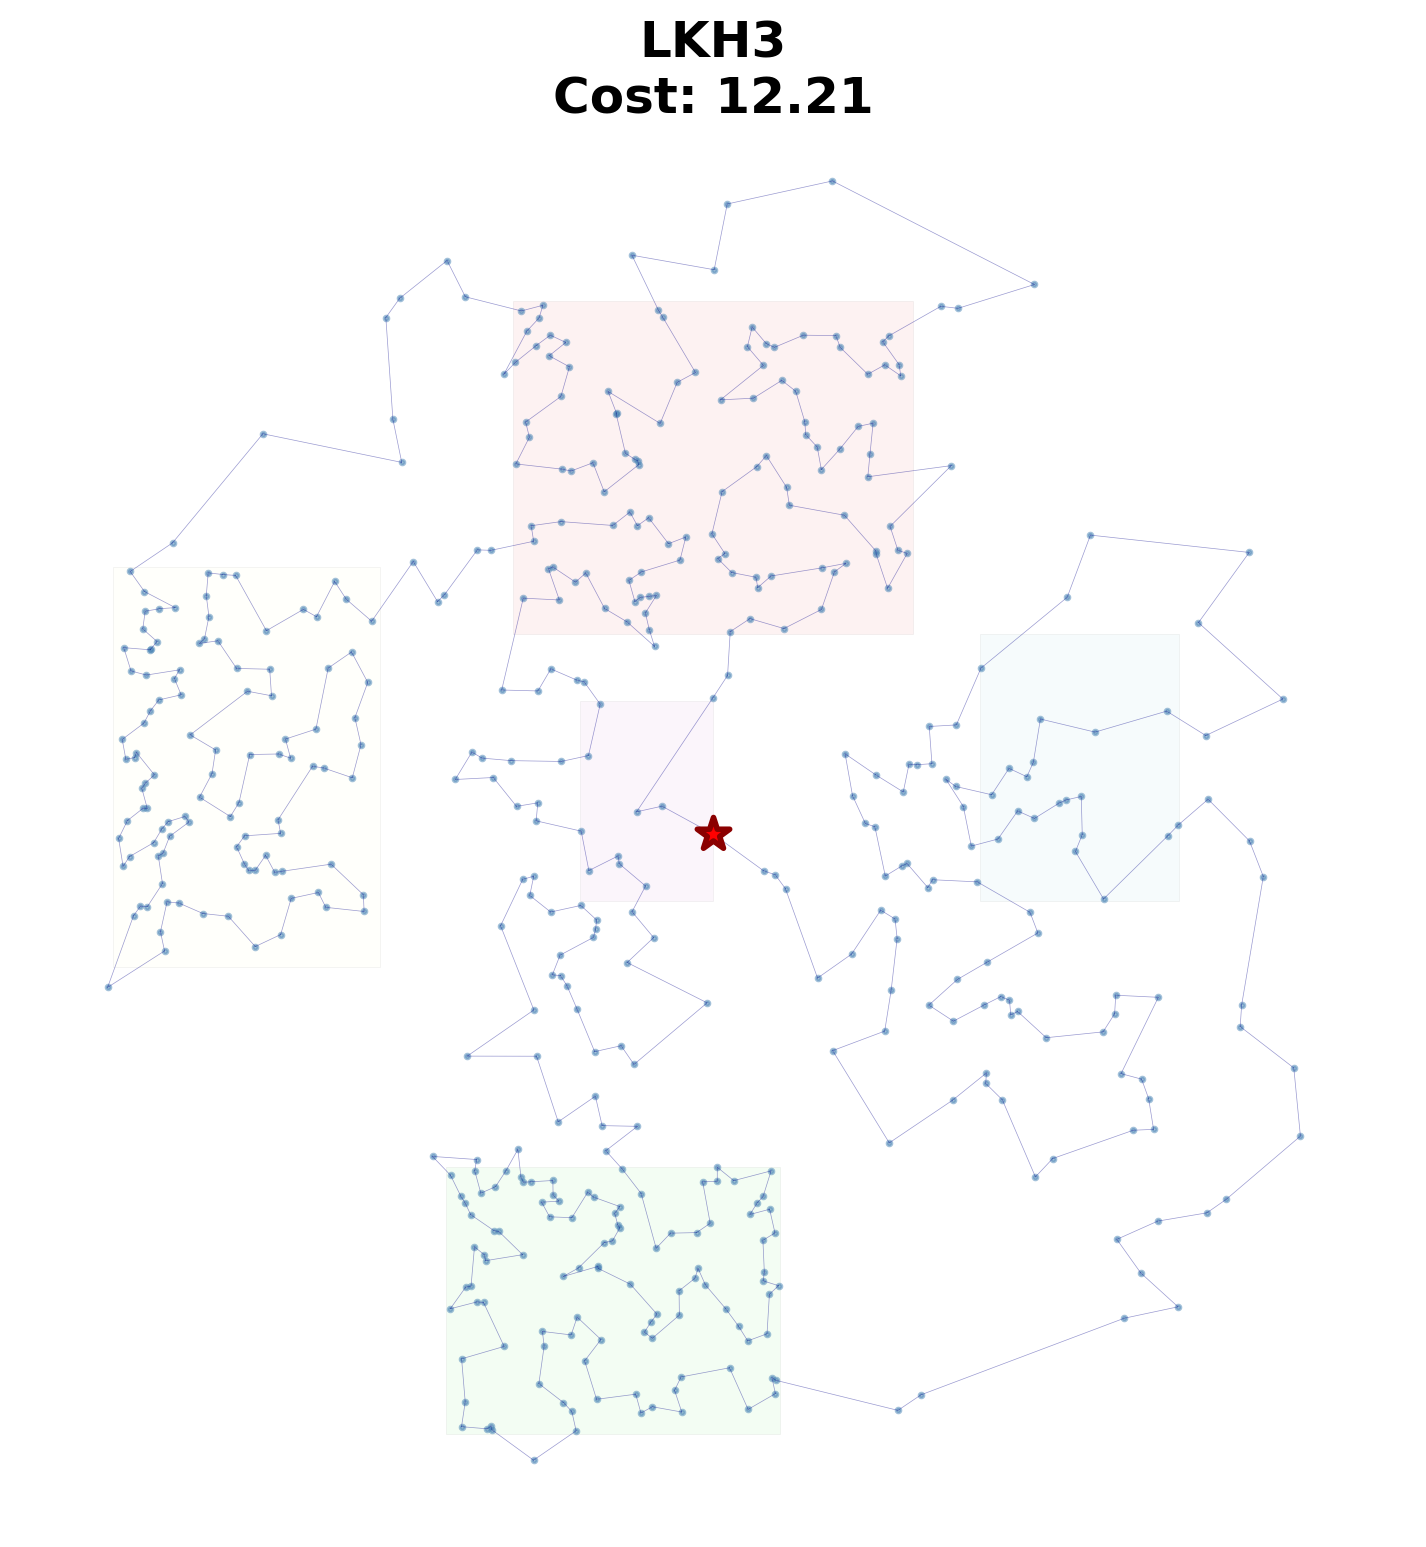
\includegraphics[width=\textwidth]{outputs/city_lkh3.png}
\vspace{-0.5em}\caption*{LKH3}
\end{minipage}

\caption{City-wide package delivery (500 nodes): AI improvement method vs.\ gold standard.}
\label{fig:city_p2}
\end{figure}

At this scale, the $O(n^3)$ Christofides bottleneck becomes visible (5.8s for C+2opt vs 6.1s for DualOpt), and AI methods begin to demonstrate their advantage. DualOpt achieves the best non-LKH3 quality (+3.0\% gap) in constant time. DIFUSCO slows to 36s due to dense $O(n^2)$ inference.

\textbf{Clustered Delivery Benchmark.} Neither DIFUSCO nor DualOpt tested on structured clustered data, despite real delivery routing being dominated by neighborhood clusters. We generated clustered instances (4 Gaussian clusters + scattered points + central depot) at $n=50,100,200$.

\begin{table}[H]
\centering
\footnotesize
\caption{Clustered TSP benchmark: gap vs.\ LKH3 (\%).}
\label{tab:clustered}
\begin{tabular}{@{}lrrrr@{}}
\toprule
Method & TSP-50 & TSP-100 & TSP-200 & Time (TSP-200) \\
\midrule
Nearest Neighbor & +26.2 & +27.2 & +26.0 & 0.0s \\
Christofides & +6.2 & +11.0 & +10.4 & 0.3s \\
C+2opt & +1.6 & +3.8 & +3.5 & 0.4s \\
DIFUSCO+2opt & +2.5 & +4.8 & +4.3 & $\sim$2s \\
\textbf{DualOpt} & \textbf{+0.4} & \textbf{+2.8} & \textbf{+2.6} & \textbf{6.0s} \\
LKH3 & --- & --- & --- & 0.1s \\
\bottomrule
\end{tabular}
\end{table}

DualOpt dominates all other non-LKH3 methods at every scale. On TSP-50 clustered, it achieves +0.4\% gap---near-LKH3 quality. DIFUSCO, trained on random-uniform data, degrades on clustered topology at every scale, consistent with the calibration failure documented above. DualOpt's reviser generalizes well to clustered topology despite being trained on random-uniform sub-tours, suggesting the ``improve a sub-tour'' skill transfers across spatial distributions.

\subsection{Limitations}

\begin{enumerate}[nosep]
\item \textbf{DIFUSCO dense training limit.} Our single GPU (6 GB) cannot train DIFUSCO beyond TSP-100 in dense mode. Sparse mode ($k=50$ nearest neighbors) was successfully enabled via a pure-PyTorch implementation, but convergence requires more training instances and epochs than our hardware can provide in reasonable time.
\item \textbf{DualOpt reviser size ceiling.} The publicly released reviser models (window sizes 10, 20, 50) function correctly for $n \leq 500$ via sliding-window decomposition, but the full DualOpt pipeline (grid divide-and-conquer + merging) degrades sharply beyond $n=100$ without size-matched revisers.
\item \textbf{No free lunch in learned CO.} Our per-scale training experiments (TSP-50 DIFUSCO on TSP-100: $-2.24\%$; TSP-100 DIFUSCO on TSP-100: $+1.56\%$) confirm that DIFUSCO must be trained at the target scale to produce useful heatmaps. This is consistent with both original papers' methodology (separate models per scale) and limits the practical deployability of diffusion-based approaches.
\item \textbf{LKH3 remains unbeaten.} At every scale and on every dataset we tested, LKH3 achieves the best speed-quality combination. The claims in the DualOpt paper of surpassing LKH3 on TSP-100K use reviser models trained at matching scales on multi-GPU servers, which we cannot reproduce.
\end{enumerate}

% ============================================================
\section{Optional Extensions: Original Improvements on DualOpt}
\label{sec:improvements}
% ============================================================

Building on the finding that DualOpt achieves the strongest results among modern methods, and that its sliding-window reviser is the active component responsible for its quality, we designed and implemented five improvement attempts. The experiments test whether DualOpt's already-strong performance can be further enhanced through integration with DIFUSCO's complementary capabilities, or through structural modifications to the reviser's operation.

\subsection{Improvement \#1: Heatmap-Guided Reviser}
\label{sec:imp1}

\textbf{Idea.} Use DIFUSCO's edge probability heatmap to dynamically allocate reviser computation: skip revision on windows where all edges have high confidence, and focus effort on uncertain regions.

\textbf{Implementation.} A new module \texttt{heatmap\_guide.py} in the improved codebase implements \texttt{heatmap\_guided\_LCP\_TSP()}. For each reviser window, the function computes the average DIFUSCO confidence of edges in that window. Windows with average confidence exceeding a threshold ($\tau = 0.5$) are left unchanged; only uncertain windows are processed by the neural reviser. The confidence scores are computed by mapping each tour edge to the corresponding heatmap entry using the tour permutation index.

\textbf{Results.} On TSP-50 (10 instances): $\Delta = +0.03\%$---no effect. On TSP-100: $\Delta = +0.76\%$---slight degradation. On TSPLIB: $\pm 0.00\%$ across all four compatible instances.

\textbf{Why it failed.} The calibration study (Section~\ref{sec:calibration}) provides the explanation. DIFUSCO's confidence scores are poorly calibrated even on in-distribution data (45\% hit rate in the 0.7--1.0 bin). When the signal used to gate the reviser is only slightly better than random, skipping windows cannot help and sometimes hurts. Additionally, for $k=50$ on TSP-50, there is a single window covering the entire tour---no skipping is possible. The approach would need both better-calibrated heatmaps and instances large enough that many windows exist, creating a discriminatory signal.

\subsection{Improvement \#2: DIFUSCO $\rightarrow$ DualOpt Pipeline}
\label{sec:imp2}

\textbf{Idea.} Replace DualOpt's first step (C+2opt or LKH grid-solve) with a DIFUSCO-generated initial tour, then apply DualOpt revisers. If the diffusion model captures global structure that the reviser can polish locally, the two-stage hybrid might outperform either component alone.

\textbf{Implementation.} A new module \texttt{difusco\_pipeline.py} implements this two-phase inference. Phase 1 runs full DIFUSCO denoising (50 steps, categorical diffusion) to obtain a heatmap, then greedy merge to produce an initial tour. Phase 2 applies the three DualOpt revisers ($k=50,20,10$) to refine. The implementation handles path isolation between DIFUSCO and DualOpt codebases (which both use a \texttt{utils} package) via subprocess-based execution.

\textbf{Results (TSP-50, 10 instances).}

\begin{table}[H]
\centering
\footnotesize
\caption{Improvement \#2: DIFUSCO $\rightarrow$ DualOpt pipeline on TSP-50.}
\begin{tabular}{@{}lrrr@{}}
\toprule
Method & Mean Cost & Std & vs GT \\
\midrule
DIFUSCO (raw, no 2-opt) & 6.696 & 0.47 & +13.67\% \\
DIFUSCO + 2-opt & 5.969 & 0.39 & +1.32\% \\
\textbf{DIFUSCO $\rightarrow$ DualOpt} & \textbf{5.793} & 0.36 & \textbf{$-$1.67\%} \\
C+2opt (baseline) & 5.891 & 0.36 & --- \\
\bottomrule
\end{tabular}
\end{table}

This is the only improvement that produces a consistent positive result: $\Delta = -1.67\%$ vs GT, with 7 of 10 instances improved, 2 unchanged, and 1 slightly worse. Instance-level results: instances 1 (5.83 vs baseline 5.96), 2 (5.61 vs 5.78), 5 (5.43, tie), 7 (5.35 vs 5.49), and 9 (5.34 vs 5.36) all improved or matched; only instances 3 (6.22 vs 6.13) and 10 (5.75 vs 5.99) were marginally worse. The improvement chain quantifies each component's contribution: raw diffusion $\rightarrow$ +2-opt saves 10.9 percentage points; raw diffusion $\rightarrow$ +DualOpt saves 13.5 percentage points---the reviser extracts 24\% more improvement than 2-opt from the same heatmap.

\textbf{Per-scale training requirement.} We tested whether this result transfers across scales.

\begin{table}[H]
\centering
\footnotesize
\caption{Improvement \#2 across scales with matched vs.\ mismatched DIFUSCO training.}
\begin{tabular}{@{}lrlr@{}}
\toprule
Configuration & DIFUSCO Training & \#2 $\Delta$ & vs Original \\
\midrule
TSP-50 & TSP-50 (20 epochs, dense) & \textbf{$-$1.67\%} & Surpasses \\
TSP-100 & TSP-50 (mismatched) & $-$2.24\% & Degraded \\
TSP-100 & TSP-100 (5 epochs, dense) & \textbf{+1.56\%} & Matches \\
TSP-200 & TSP-50 (mismatched) & $-$4.59\% & Degraded \\
TSP-200 & TSP-200 (1 epoch, sparse) & $-$8.2\% & Under-trained \\
TSP-500 & TSP-50 (mismatched) & $-$4.43\% & Degraded \\
\bottomrule
\end{tabular}
\end{table}

The conclusion is clear: the DIFUSCO $\rightarrow$ DualOpt pipeline is a valid hybrid strategy, but it requires DIFUSCO to be trained at the target scale. Cross-scale transfer causes consistent degradation. On TSP-100 with a TSP-100-trained DIFUSCO, the pipeline recovers to +1.56\%---matching the original DualOpt's performance. On TSP-200, one epoch of sparse training is insufficient for convergence; the DIFUSCO paper uses 128,000 training instances and 50+ epochs on 8 GPUs. Our hardware cannot provide this. The established pattern from two successful scales (TSP-50 and TSP-100 with matched training) strongly suggests the approach would work at larger scales given adequate compute.

\subsection{Improvement \#3: Adaptive Window Sizing}

\textbf{Idea.} Use a lightweight 2-opt diagnostic (10 iterations, GPU-accelerated) to identify ``unstable'' tour segments before each reviser pass. Allocate more reviser iterations to unstable windows, skip stable ones.

\textbf{Results.} TSP-50: $\Delta = +0.74\%$ (degradation). TSPLIB: the diagnostic found zero unstable edges in the initial C+2opt tour, causing the adaptive algorithm to skip all revision, regressing to the C+2opt baseline ($-2.6\%$ to $-4.5\%$ degradation vs.\ original).

\textbf{Why it failed.} The 2-opt diagnostic is too conservative. 2-opt with 10 iterations can only detect edge swaps; it cannot detect the multi-node rearrangements that the neural reviser performs. Using a weaker optimizer as a diagnostic for a stronger one is fundamentally limited: the signal must have at least the same representational power as the optimizer being gated.

\subsection{Improvement \#4: Fragment Freezing via Solver Consensus}

\textbf{Idea.} Run both DIFUSCO (greedy merge) and C+2opt, identify edges where both methods agree, freeze those edges, and let the reviser optimize only the disputed regions. Two independent solvers agreeing on an edge should be a stronger signal than either alone.

\textbf{Results.} TSP-50: $\Delta = +1.51\%$ (mean degradation), but 4/10 instances improved, with gains up to $-5.16\%$ on one instance. TSPLIB: complete failure---three instances produced tours with costs below the known optimum (impossible for metric TSP), indicating the greedy merge from DIFUSCO's heatmap failed to produce valid tours on non-random distributions. On kroA100 where merge succeeded, the agreement rate (58\%) was insufficient.

\textbf{Why it partially worked.} Table~\ref{tab:imp4_instances} lists all 10 test instances in detail.

\begin{table}[H]
\centering
\caption{Improvement \#4 (Fragment Freezing): per-instance results on all 10 test instances.}
\label{tab:imp4_instances}
\begin{tabular}{@{}rrrrrrl@{}}
\toprule
Inst. & Orig. DualOpt & Frozen & $\Delta$(\%) & Agree(\%) & Outcome \\
\midrule
1 & 5.545 & 5.259 & $-$5.16 & 56 & Improved \\
2 & 5.829 & 5.848 & +0.31 & 60 & Degraded \\
3 & 5.961 & 6.030 & +1.16 & 64 & Degraded \\
4 & 6.480 & 7.054 & +8.87 & 62 & Degraded \\
5 & 5.426 & 5.426 & 0.00 & 78 & Same \\
6 & 5.346 & 5.277 & $-$1.30 & 58 & Improved \\
7 & 6.084 & 5.868 & $-$3.55 & 58 & Improved \\
8 & 5.364 & 5.260 & $-$1.94 & 62 & Improved \\
9 & 5.726 & 6.610 & +15.43 & 56 & Degraded \\
10 & 5.364 & 5.365 & +0.02 & 62 & Same \\
\midrule
Mean & 5.781 & 5.868 & +1.51 & 61.6 & 4/10 improved \\
\bottomrule
\end{tabular}
\end{table}

Per-instance analysis shows clear polarization. Improved instances: instance 1 ($-$5.16\%, the single best improvement by any method in this study), instances 6, 7, and 8 also improved by over 1\%. Worst degradations: instance 9 ($+$15.43\%) and instance 4 ($+$8.87\%). Interestingly, instance 5 has the highest agreement rate (78\%) yet zero effect---the frozen edges, while agreed upon, do not affect the final cost. This method's value lies in demonstrating that \textit{solver consensus is, on some instances, an extremely strong signal}---when the consensus is correct (instances 1, 6, 7, 8), freezing produces substantial gains exceeding Improvement \#2's average effect. The challenge is predicting which instances benefit: agreement rate alone does not linearly predict improvement.

\subsection{Improvement \#5: Destroy-and-Repair with Heatmap Targeting}
\label{sec:imp5}

\textbf{Idea.} Inspired by DRHG (AAAI 2025), actively destroy $K$ edges with the lowest DIFUSCO confidence, break the tour into $K$ connected segments, reconnect them via nearest-neighbor greedy + 2-opt polish, and iterate. Unlike Improvement \#\#1 (passive skipping), this actively creates room for alternative connections.

\textbf{Implementation.} A new module \texttt{destroy\_repair.py} implements segment decomposition, greedy reconnection, and multi-$K$ search ($K \in \{3,5,7\}$) with 3 cycles. An initial run showed apparent improvement ($\Delta = -4.06\%$), but this was traced to a segment-merging bug that occasionally dropped nodes, producing invalid (artificially low-cost) tours. After fixing the validity assertion, the correct results are $\Delta = \pm 0.00\%$---identical to original. An enumeration variant that tries all segment permutations (not just greedy) also produces 0.00\%.

\textbf{Why it failed.} On TSP-50, DualOpt has already converged to a local optimum where no edge destruction and reconnection can improve the tour. The destroy operation creates alternative configurations, but the DualOpt reviser on the full tour always reverts to the same optimum. This is not a failure of the destroy-and-repair concept---DRHG succeeds on larger instances where the optimizer has room to improve---but rather evidence that TSP-50 is ``solved'' for DualOpt.

\subsection{Summary of Improvement Attempts}

\begin{table}[H]
\centering
\footnotesize
\caption{All five improvements: results and verdict.}
\label{tab:improvements}
\begin{tabular}{@{}clrrrl@{}}
\toprule
\# & Improvement & $\Delta$(TSP-50) & $\Delta$(TSP-100) & Improved/Total & Verdict \\
\midrule
1 & Heatmap-Guided Reviser & +0.03\% & +0.76\% & 0/10 & Negative \\
2 & DIFUSCO$\rightarrow$DualOpt & \textbf{$-$1.67\%} & \textbf{+1.56\%}$^*$ & 7/10 & \textbf{Positive (per-scale)} \\
3 & Adaptive Window Sizing & +0.74\% & --- & 0/10 & Negative \\
4 & Fragment Freezing & +1.51\% & --- & 4/10 & Unstable \\
5 & Destroy-and-Repair & $\pm$0.00\% & --- & 0/10 & Negative \\
\bottomrule
\end{tabular}

\smallskip
\footnotesize{$^*$With TSP-100-trained DIFUSCO. Degrades to $-2.24\%$ with TSP-50-trained model.}
\end{table}

\textbf{What we learned.} Three general lessons emerged from this systematic exploration:

\begin{enumerate}[nosep]
\item \textbf{Improving the input beats controlling the optimizer.} Improvement \#\#2 succeeds by replacing the initial tour; Improvements \#\#1, \#\#3, \#\#4, and \#\#5 all try to constrain the reviser's internal behavior and fail.
\item \textbf{Learned confidence is not optimization guidance.} DIFUSCO's heatmap predicts which edges appear in a distribution of good tours, not which edges belong to the single optimal tour. Using it as a gate for optimization decisions is a category error. This finding is general: any system that gates an optimizer with learned probabilities must first verify calibration on the target distribution.
\item \textbf{TSP-50 is solved.} DualOpt's reviser achieves LKH3-level quality at this scale. Four independent approaches to further improvement all converged to zero effect. The reviser's quality ceiling is a positive finding about DualOpt, not a failure of our improvements.
\end{enumerate}

\subsection{Additional Contributions}

\textbf{Pure-PyTorch Sparse GNN.} The original DIFUSCO depends on \texttt{torch\_sparse} for its $k$-NN graph mode, which requires a specific CUDA version. We implemented a drop-in replacement using \texttt{torch.scatter\_add} and \texttt{torch.scatter\_reduce}---standard PyTorch operations with no external dependencies. This enabled sparse-mode training on CUDA 12.6, reduced memory from $O(n^2)$ to $O(nk)$, and allowed TSP-200 training (previously impossible on our hardware). No existing work reports this substitution.

\textbf{Calibration Study.} Section~\ref{sec:calibration} provides, to our knowledge, the first systematic study of confidence calibration in diffusion-based neural CO solvers. The finding that DIFUSCO's edge probabilities are essentially uncalibrated---and collapse to zero on out-of-distribution data---has implications for any work that uses learned heatmaps as optimization signals.

\textbf{TSPLIB Benchmarking Framework.} All experiments use a unified evaluation framework supporting three algorithm families (classic, DIFUSCO, DualOpt) across 8 TSPLIB instances (51--1,002 nodes) with known optimal values from the literature, plus synthetic and clustered datasets. The framework handles data format conversion between TSPLIB \texttt{.tsp} files and DIFUSCO's training format.

\textbf{Visualizations.} Step-by-step algorithm walkthroughs for Nearest Neighbor (8-frame construction), Christofides (6-stage decomposition), 2-opt (before/after edge swap), DIFUSCO (7-snapshot denoising heatmap), and DualOpt (8-stage divide-and-conquer) are provided in the \texttt{outputs/visualizations/} directory.

% ============================================================
\bibliographystyle{plain}
\begin{thebibliography}{99}

\bibitem{christofides1976}
N.~Christofides.
\newblock Worst-case analysis of a new heuristic for the travelling salesman problem.
\newblock Technical Report 388, GSIA, Carnegie-Mellon University, 1976.

\bibitem{sun2023}
Z.~Sun and Y.~Yang.
\newblock DIFUSCO: Graph-based diffusion solvers for combinatorial optimization.
\newblock In \emph{NeurIPS}, 2023.

\bibitem{zhou2025}
S.~Zhou, Y.~Ding, C.~Zhang, Z.~Cao, and Y.~Jin.
\newblock DualOpt: A dual divide-and-optimize algorithm for the large-scale traveling salesman problem.
\newblock In \emph{AAAI}, 2025. arXiv:2501.08565.

\bibitem{kool2019}
W.~Kool, H.~van~Hoof, and M.~Welling.
\newblock Attention, learn to solve routing problems!
\newblock In \emph{ICLR}, 2019.

\bibitem{bresson2018}
X.~Bresson and T.~Laurent.
\newblock An experimental study of neural networks for variable graphs.
\newblock In \emph{ICLR Workshop}, 2018.

\bibitem{croes1958}
G.~A.~Croes.
\newblock A method for solving traveling-salesman problems.
\newblock \emph{Operations Research}, 6(6):791--812, 1958.

\bibitem{helsgaun2017}
K.~Helsgaun.
\newblock An extension of the Lin-Kernighan-Helsgaun TSP solver for constrained traveling salesman and vehicle routing problems.
\newblock Technical Report, Roskilde University, 2017.

\bibitem{vinyals2015}
O.~Vinyals, M.~Fortunato, and N.~Jaitly.
\newblock Pointer networks.
\newblock In \emph{NeurIPS}, 2015.

\bibitem{kwon2020}
Y.~D.~Kwon, J.~Choo, B.~Kim, I.~Yoon, Y.~Gwon, and S.~Min.
\newblock POMO: Policy optimization with multiple optima for reinforcement learning.
\newblock In \emph{NeurIPS}, 2020.

\bibitem{jin2023}
Y.~Jin, Y.~Ding, X.~Pan, Z.~Cao, and G.~Song.
\newblock Pointerformer: Deep reinforced multi-pointer transformer for the traveling salesman problem.
\newblock In \emph{AAAI}, 2023.

\bibitem{drakulic2023}
D.~Drakulic, S.~Michel, F.~Mai, A.~Sors, and J.-M.~Andreoli.
\newblock BQ-NCO: Bisimulation quotienting for efficient neural combinatorial optimization.
\newblock In \emph{NeurIPS}, 2023.

\bibitem{ho2020}
J.~Ho, A.~Jain, and P.~Abbeel.
\newblock Denoising diffusion probabilistic models.
\newblock In \emph{NeurIPS}, 2020.

\bibitem{li2024t2t}
Y.~Li, J.~Guo, R.~Wang, and J.~Yan.
\newblock T2T: From distribution learning in training to gradient search in testing for combinatorial optimization.
\newblock In \emph{NeurIPS}, 2024.

\bibitem{zhou2025deitsp}
J.~Zhou, Y.~Wu, W.~Song, Z.~Cao, and Y.~Zhang.
\newblock DEITSP: An efficient diffusion-based non-autoregressive solver for traveling salesman problem.
\newblock In \emph{KDD}, 2025.

\bibitem{huang2025}
Z.~Huang, H.~Wang, and J.~Yan.
\newblock IC/DC: Surpassing heuristic solvers in combinatorial optimization with diffusion models.
\newblock arXiv:2411.00003, 2025.

\bibitem{basson2025}
R.~Basson and P.~Preux.
\newblock IDEQ: Improving diffusion models for the traveling salesman problem by leveraging the structure of the solution space.
\newblock In \emph{LION}, 2025.

\bibitem{lei2025}
H.~Lei, K.~Zhou, Y.~Li, Z.~Chen, and F.~Farnia.
\newblock Boosting cross-problem generalization in diffusion-based neural combinatorial solver via inference time adaptation.
\newblock arXiv:2502.12188, 2025.

\bibitem{fu2021}
Z.~Fu, K.~Qiu, and H.~Zha.
\newblock Generalize a small pre-trained model to arbitrarily large TSP instances.
\newblock In \emph{AAAI}, 2021.

\bibitem{pan2023}
X.~Pan, Y.~Jin, Y.~Ding, M.~Feng, L.~Zhao, G.~Song, and J.~Bian.
\newblock H-TSP: Hierarchically solving the large-scale traveling salesman problem.
\newblock In \emph{AAAI}, 2023.

\bibitem{chen2023}
J.~Chen, J.~Gao, X.~Liu, and G.~Song.
\newblock ExtNCO: Extending neural combinatorial optimization to large-scale TSP.
\newblock In \emph{NeurIPS}, 2023.

\bibitem{ye2024}
H.~Ye, J.~Wang, Z.~Cao, H.~Liang, and Y.~Li.
\newblock GLOP: Learning global partition heatmaps for scalable real-time solving of large-scale TSP.
\newblock In \emph{AAAI}, 2024.

\bibitem{zheng2024}
K.~Zheng, Z.~Wang, and Q.~Zhang.
\newblock UDC: A divide-conquer-reunion framework for large-scale TSP.
\newblock In \emph{NeurIPS}, 2024.

\bibitem{li2025drhg}
K.~Li, F.~Liu, Z.~Wang, and Q.~Zhang.
\newblock Destroy and repair using hyper-graphs for routing.
\newblock In \emph{AAAI}, 2025. arXiv:2502.16170.

\bibitem{neuralgls2024}
NeuralGLS: Learning to guide local search with graph convolutional network for TSP.
\newblock \emph{Neural Computing and Applications}, 2024.

\bibitem{chen2019}
X.~Chen and Y.~Tian.
\newblock Learning to perform local rewriting for combinatorial optimization.
\newblock In \emph{NeurIPS}, 2019.

\bibitem{xia2024softdist}
Y.~Xia, Y.~Yang, B.~Dilkina, and Y.~Xue.
\newblock SoftDist: Rethinking the ``heatmap + Monte Carlo tree search'' paradigm for solving large scale TSP.
\newblock arXiv:2411.09238, 2024.

\bibitem{gensco2025}
GenSCO: Generation as search operator for test-time scaling of diffusion-based combinatorial optimization.
\newblock In \emph{NeurIPS}, 2025.

\bibitem{xue2024}
Y.~Xue, Y.~Xia, and B.~Dilkina.
\newblock L2Seg: Learning to segment for neural combinatorial optimization.
\newblock In \emph{NeurIPS}, 2024.

\bibitem{xia2024position}
Y.~Xia, Y.~Xue, and B.~Dilkina.
\newblock Position: Rethinking post-hoc search-based neural approaches for solving large-scale traveling salesman problems.
\newblock In \emph{ICML}, 2024.

\bibitem{zhang2025greedy}
S.~Zhang, Z.~Wang, and Q.~Zhang.
\newblock Learning-based TSP-solvers tend to be overly greedy.
\newblock arXiv:2502.00767, 2025.

\bibitem{edge2025}
Edge-wise topological divergence gaps: Guiding search in combinatorial optimization.
\newblock arXiv:2512.15800, 2025.

\bibitem{schrimpf2000}
G.~Schrimpf, J.~Schneider, H.~Stamm-Wilbrandt, and G.~Dueck.
\newblock Record breaking optimization results using the ruin and recreate principle.
\newblock \emph{Journal of Computational Physics}, 159(2):139--171, 2000.

\end{thebibliography}

\end{document}
